\documentclass[12pt]{report}
\usepackage[utf8x]{inputenc}
\usepackage[english]{babel}
\usepackage[pdftex]{graphicx}
\usepackage[T1]{fontenc}
\usepackage{color}
\usepackage{wrapfig}
\usepackage{amsmath}
\usepackage{amssymb}
\usepackage{textcomp}
\usepackage{array}
\usepackage{booktabs}
\usepackage{subfigure}
\usepackage[font=small,format=plain,labelfont=bf,up,textfont=it,up]{caption}
\usepackage{longtable}
\usepackage{calc}
\usepackage{setspace}
\usepackage{multirow}
\usepackage{hhline}
\usepackage{ifthen}
\usepackage{lscape}
\usepackage{relsize}
\usepackage{bbold}
\usepackage{mathtext}
\usepackage{pdfpages}
\usepackage{geometry}
 \geometry{
 a4paper,
 total={170mm,257mm},
 left=35mm,
 top=25mm,
 bottom=25mm,
 right=20mm,
 }
\usepackage{cite}
\renewcommand{\chaptername}{}
\linespread{1.3}

\graphicspath{ {FIGURES/} }
\begin{document}

\tableofcontents

\chapter*{Overview}
\addcontentsline{toc}{chapter}{Overview}
The program is intended to aid calculation of properties using multi-reference perturbation theory,
and to provide a computationally efficient means of handling the very large data structures 
and complex expressions associated with such methods. Essentially, this involves
having a generic interface for evaluating expressions of the form
\begin{equation}
\langle M | \hat{X} \hat{Y} ... | N \rangle,
\label{eqn:basic}
\end{equation}
\noindent where $\hat{X}$ and $\hat{Y}$ are some arbitrary operators, and $| N
\rangle$  is a multireference wavefunction represented as a linear combination
of determinants, $|I\rangle $;
\begin{equation}
|N\rangle = \sum_{I} c_{I}^{N}| I \rangle.
\end{equation} 
\noindent Written using second quantization (\ref{eqn:basic}) would be
\begin{equation}
\sum_{\substack{ x_{1}x_{2}...\\ y_{1}y_{2}... \\ ...}} X_{x_{1}x_{2}...} Y_{y_{1}y_{2}...} ...
\sum_{I}\sum_{J}
\langle I | a^{\dagger}_{x_{1}} a_{x_{2}}...a^{\dagger}_{y_{1}}a_{y_{2}}....| J \rangle 
 c^{M \dagger}_{I}c^{N}_{J}.
\label{eqn:basic_2nd_quantized}
\end{equation}
\noindent  Here, $X_{x_{1},x_{2}...}$ and $Y_{y_{1},y_{2}...}$ are just representations of operators 
$\hat{X}$ and $\hat{Y}$ in the molecular orbital basis.\\

\noindent It is also possible to calculate derivatives of (\ref{eqn:basic_2nd_quantized})  with respect to CI-coefficients, $c_{I}^{N}$;
\begin{equation}
\sum_{\substack{ x_{1}x_{2}...\\ y_{1}y_{2}... \\ ...}} X_{x_{1}x_{2}...} Y_{y_{1}y_{2}...} ...
\sum_{J}
\langle I | a^{\dagger}_{x_{1}} a_{x_{2}}...a^{\dagger}_{y_{1}}a_{y_{2}}....| J \rangle 
c^{N}_{J}
\label{eqn:ci_derivative}
\end{equation}
\noindent In a similar vein, it is possible to evaluate expressions of form:
\begin{equation*}
\sum_{\substack{ x_{1}x_{2}...\\ y_{1}y_{2}... \\ ...}} X_{x_{1}x_{2}...} Y_{y_{1}y_{2}...} ...
\sum_{\Omega}
\sum_{I}\sum_{J}
\langle I | \hat{E}^{\dagger}_{\Omega} a^{\dagger}_{x_{1}} a_{x_{2}}...a^{\dagger}_{y_{1}}a_{y_{2}}....| J \rangle 
 c^{M \dagger}_{I}c^{N}_{J}
\end{equation*}
\begin{equation}
=
\sum_{\substack{ x_{1}x_{2}...\\ y_{1}y_{2}... \\ ...}} X_{x_{1}x_{2}...} Y_{y_{1}y_{2}...} ...
\sum_{I}\sum_{J}
\langle I | a_{\omega_{1}} a_{\omega_{2}}.. .a^{\dagger}_{x_{1}} a_{x_{2}}...a^{\dagger}_{y_{1}}a_{y_{2}}....| J \rangle 
 c^{M \dagger}_{I}c^{N}_{J}
\label{eqn:basic_2nd_quantized_projector}
\end{equation}
\noindent where the $\hat{E}^{\dagger}_{\Omega}$ is a projection operator
which excites electrons into the virtual space, from the orbitals used to construct
the space in which the reference wavefunctions, $\{|N\rangle\}$, were originally defined.\\

\noindent The program is intended to be flexible; and instead of asking for
specific perturbation theories or properties the user has the option of
specifying algebraic expressions directly via the input file.\\

\noindent It is important to note that the program is intended to facilitate property 
calculations on wavefunctions obtained from multireference calculations. Hence it
is necessary to first run a CASSCF calculation before calling the program. Furthermore,
the program does not contain routines for evaluation of molecular orbital integrals;
when such integrals are needed it calls to the pre-existing routines in the 
Bagel~\cite{BAGEL} code.

\section{Structural outline}
\noindent The program is split into three main components; an algebraic manipulator, an FCI
iand linear algebra library (mainly consisting of routines for performing tensor contractions),
and a task translation module for facilitating communication between these two components.\\

\begin{figure}[!ht]
\begin{center}
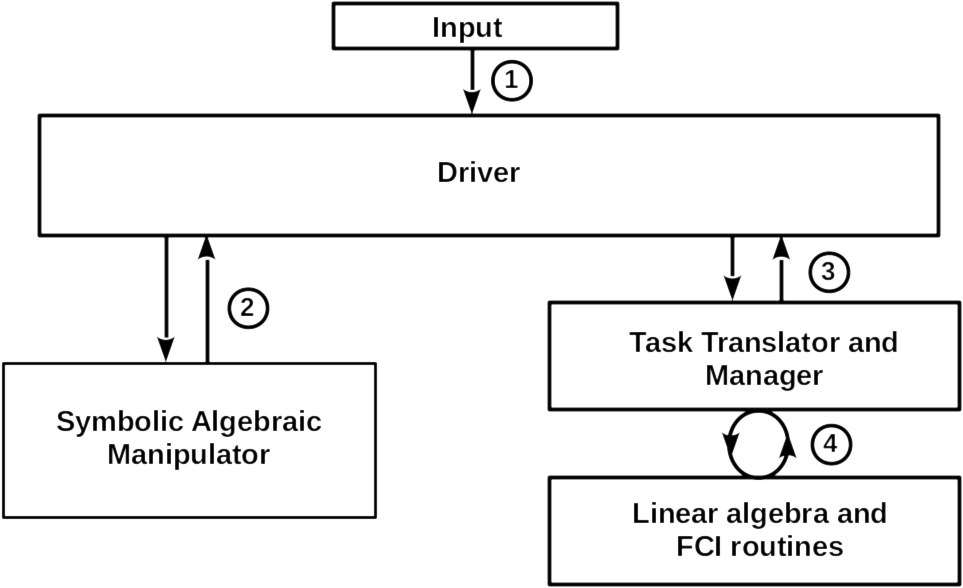
\includegraphics[width=0.8\textwidth]{prog_structure.png}
\caption{ Outline of program structure. Arrows represent the flow of data, numbers represent the
initial order in which the components are used (looping may occur in the case of iterations).
The intention is that each component, with the exception of the driver, functions independently of the others.}
\end{center}
\label{fig:prog_structure}
\end{figure}

\noindent The algebraic manipulator interprets the expressions defined
in the input, and restructures them into a number of quantities which are
more suited to computational evaluation. To accomplish this the
algebraic manipulator makes extensive use of the commutation
relations of the creation and annihilation operators, as well as the physical
symmetries of the operators, in order to minimize the number of terms, and
avoid the need for calculation of terms which are likely to be computationally
expensive to evaluate (e.g., those with large numbers of indexes). This series
of expressions is used to form an algebraic task list; a sequence of
generic mathematical operations which are evaluated by other parts of the program.
It is important to note that the algebraic manipulator is entirely based around symbolic manipulation,
and does not handle any of the large data structures, e.g., CI-vectors,
molecular orbital integral tensors, etc.. The expressions in the algebraic
task list do not in any way specify what kind of data structures need to
be used to store the quantities necessary for their evaluation.\\

\noindent The FCI and tensor libraries contain generic routines for calculating
density matrices and their derivatives, and performing tensor contractions and
various other tensor manipulations. The tensor and FCI library are completely
seperate from the symbolic algebraic manipulator, and operate totally independently. The
routines within the FCI library have a recursive structure, which 
enables calculation of density matrices (and
derivatives) of arbitrary order. In a similar vein, the tensor library can
operate on tensors of arbitrary order, with each dimension being a different
size. At present the FCI  library uses the Determinant class defined in
Bagel~\cite{BAGEL}. The tensor libraries make use of the SMITH::Tensor class
defined in Bagel, which in turn makes use of the TiledArray~\cite{TiledArray}
libraries for parallel storage of the data.  The routines in the tensor
arithmetic library are built using a combination of calls to
LAPACK~\cite{LAPACK}, and the tensor transposition routine defined in
TiledArray\footnote{ To clarify, whilst TiledArray has some tensor contraction
routines, these were found to not be suitable for the current purpose, and are
not used.}.\\

\noindent The final major component of the program is the task translator,
which faciliates communication between the algebraic manipulator and the 
FCI and tensor libraries. This is necessary, as
neither the arithmetic component has knowledge of the classes used in
the algebraic manipulator, and vice versa. Whilst this has complicated the
design slightly, it should enable greater portability, as well as making the
program substantially easier to extend and upgrade.\\ 

\noindent In a sense there is a fourth component, a driving routine, which
performs some communication between the three routines, parsing of the input,
and some initialization. However, whilst this component is practically
important, and not particularly small, it is rather simple and of little
interest, so I will not discuss it significantly.

\section{Specific components}
The functioning of the program is best explained by example. In the following,
use of italicized words indicate that word is a class defined in the program.
The "highest level" class is the \emph{equation}, which determines what the
final output of the program is. For example, the user may ask the program to find the 
$\hat{T}^{LN}$ which satisfy 
\begin{equation}
\sum_{N} 
\langle M | \hat{E}^{\dagger}_{\Omega} (\hat{H}-\epsilon_{L}) \hat{T}^{LN} | N \rangle  +
\langle M | \hat{E}^{\dagger}_{\Omega} \hat{H} | L  \rangle = 0 \text{ \ \ \ \ } \forall \text{ \ \ }  M . 
\label{eqn:eqn_example}
\end{equation}
\noindent To accomplish this, the user will specify the equation in the input file, and the 
program will use the information to construct an \emph{equation} object. This is \emph{equation}
is then used to generate a number of \emph{expression} objects, which can be evaluated independently. 
For the equation specified by (\ref{eqn:eqn_example}) these \emph{expression} objects
may correspond to quantities such as
\begin{equation}
\sum_{N} 
\langle M | \hat{E}^{\dagger}_{\Omega} (\hat{H}-\epsilon_{L}) \hat{T}^{LN} | N \rangle  +
\langle M | \hat{E}^{\dagger}_{\Omega} \hat{H} | L  \rangle.
\label{eqn:Hylleras}
\end{equation}
\noindent Each \emph{equation} contains a number of such \emph{expression} objects, along with
information regarding how they relate to one another and the quantity requested by the user.
In a single instance of the \emph{expression} class corresponding to (\ref{eqn:Hylleras}),
the values of $L$ and $M$  would be set, whilst the range of
summation over $N$ would be defined. Typically, an \emph{equation} will contain many \emph{expressions}, but
these will only differ from one another by the values of the indices, or the 
constraints placed on the ranges of summations. This is to aid in parallelization;
the intention being that seperate expressions may be evaluated entirely independently from one another.\\

\noindent Each \emph{expression} is further broken down into a number of \emph{term}s.
\emph{Terms} differ from \emph{expressions} in that any state index summation in
in a \emph{term} applies to the entire term.
Hence (\ref{eqn:Hylleras}) cannot be represented by a single term object, and instead
requires two:
\begin{equation}
\sum_{N} 
\langle M | \hat{E}^{\dagger}_{\Omega} (\hat{H}-\epsilon_{L}) \hat{T}^{LN} | N \rangle  
\label{eqn:Hylleras1}
\end{equation}
\begin{equation}
\langle M | \hat{E}^{\dagger}_{\Omega} \hat{H} | L  \rangle  
\label{eqn:Hylleras2}
\end{equation}
\noindent Without this separation (\ref{eqn:Hylleras2}) would be summed over $N$ times,
despite the fact $N$ does not occur. 
Whilst this constraint seems needless and annoying there are justifications for them stemming
from the strategies, to be elaborated upon later in this document, used to merge different \emph{term}s together. \\ 

\noindent Each \emph{term} is further broken down into a list of \emph{braket}s. The \emph{term} 
in (\ref{eqn:Hylleras1}) would be broken down into $2N$ \emph{brakets}: 
\begin{equation}
\langle M | \hat{E}^{\dagger}_{\Omega} \hat{H} \hat{T}^{LN} | N \rangle  
\end{equation}
\begin{equation}
\langle M | \hat{E}^{\dagger}_{\Omega} (-\epsilon_{L}) \hat{T}^{LN} | N \rangle  
\end{equation}
\noindent Within a \emph{braket} the values of all the indexes are specified.
A single \emph{braket} consists of a bra and a ket, surrounding some many electron 
operator formed from the product of an arbitrary number of 1- and 2-electron operators.  The
individual \emph{braket}s comprising a \emph{term} are never\footnote{Excepting
the situation where a \emph{term} consists of a single \emph{braket}.}
evaluated independently; the arithmetic operations to evaluate \emph{braket}s
with common bra and ket will be merged together, provided these bra and ket
exist within the same term. Similarly, it is also possible to merge the compute
lists associated with different \emph{term}s together, though not the
\emph{term} objects themselves. However, this is not done by default, as
typically it is useful to store and evaluate \emph{term}s independently.\\

\noindent The remaining fundamental classes are the \emph{TensOps}, which contain
information regarding the second-quantized presentation of the operators, e.g.,
the tensor $\mathbf{H}$, with elements $H_{ijkl}$, where $i, j, k$ and $l$ are
molecular orbital indices. And the \emph{StatesInfo}, \emph{CIVecInfo}
classes, which contains information about which ci-sectors are used to represent the 
wavefunction, and which orbitals were used to construct these ci-sectors,  respectively.\\

\noindent The above described components are the targets upon which the 
algebraic manipulation routines act to generate the algebraic task list.  


\chapter{Tensors decomposition and contraction}
\section { Block symmetry and sparsity }

Some blocks of the tensor can be obtained by transforming other blocks. How the program exploits this is best explained
through a series of examples.\\ 

\noindent Consider two tensor blocks $Q^{b1}$ and $Q^{b2}$ between which there is the relation
\begin{equation}
Q^{b1}_{ijkl} = Q^{b2}_{ijlk}\rho,
\label{eqn:Qsymm}
\end{equation}
where $b1 = B^{\xi\xi\chi\xi }$, $b2 := B^{\xi\xi\xi\chi }$, and $\rho$ is some constant factor. This is a special case were the ranges $r^{\xi}$ and $r^{\chi}$ have
the same length:
\begin{equation}
\text{card}(r^{\xi}) = \text{card}(r^{\chi}).
\end{equation}
This case regularly occurs when dealing with spin symmetry. Here an element of block $Q^{b1}$ is equal to an element of block $Q^{b2}$ with the last two indexes interchanged.
Therefore, we do not need to store both blocks; operations on $Q^{b2}$ are equivalent to operations on $Q^{b1}$ preceded by a transformation.\\

\noindent Now consider a third, unrelated tensor block $R^{b3}$, where $b3 := \{\xi, \xi, \chi, \xi, \nu, \nu \}$. 
This tensor block is large, and $r^{\nu}$ has far greater extent than $r^{\chi}$, i.e.,
\begin{equation}
\text{card}(r^{\nu}) \gg \text{card}(r^{\chi})
\end{equation}

\noindent For example, consider calculation of elements of a tensor $\mathbf{X}$ from contractions between tensors $\mathbf{Q}$ and $\mathbf{R}$;
\begin{equation}
X_{mn} = \sum_{ijkl} Q^{b1}_{ijkl} R_{ijklmn}+ \sum_{ijkl} R^{b3}_{ijlkmn}Q^{b2}_{ijkl}.
\label{eqn:Xexample}
\end{equation} 
Note that the $l$ and $k$ indexes on $R$ have been interchanged. \\

\noindent A straight forward way to calculate this is by the following two tasks:
\begin{equation*}
\text{task A1\ : \ \ \  \ } X_{mn} = \sum_{ijkl}  Q^{b1}_{ijkl}R^{b3}_{ijklmn},
\end{equation*}                                                             
\begin{equation*}                                                           
\text{task A2\ : \ \ \  \ } X_{mn} += \sum_{ijkl} Q^{b2}_{ijlk}R^{b3}_{ijklmn}.
\end{equation*}
where the indexes on $Q^{b2}$ have been swapped to avoid the swapping the indexes on $R$.
Applying symmetry we end up with three tasks, but don't need to store $Q^{b2}$, i.e., 
\begin{equation*}
\text{task B1\ : \ \ \  \ } X_{mn} = \sum_{ijkl}  Q^{b1}_{ijkl}R^{b3}_{ijklmn}
\end{equation*}                                                             
\begin{equation*}                                                           
\text{task B2\ : \ \ \  \ } Q^{b2}_{ijkl} = - (\text{swap}(k,l)[ Q^{b1}_{ijkl}])
\end{equation*}
\begin{equation*}                                                           
\text{task B3\ : \ \ \  \ } X_{mn} += \sum_{ijkl} Q^{b2}_{ijkl}R^{b3}_{ijlkmn}
\end{equation*}
However, this saves on storage, not computation time. A better approach would be
\begin{equation*}                                                           
\text{task D1\ : \ \ \  \ } A^{b1}_{ijkl} =  Q^{b1}_{ijkl} + \rho(\text{swap}(k,l)[Q^{b1}_{ijkl}] ) 
\end{equation*}
\begin{equation*}                                                           
\text{task D2\ : \ \ \  \ } X_{mn} = \sum_{ijkl} A^{b1}_{ijkl}R^{b3}_{ijklmn}.
\end{equation*}
This could be improved even further to
\begin{equation*}                                                           
\text{task E1\ : \ \ \  \ } X_{mn} = \sum_{ijkl} (1+\rho) Q^{b1}_{ijkl}R^{b3}_{ijklmn}.
\end{equation*}
\noindent Getting to this final task list, containing just task E1, can be
extremely beneficial, not only because we can often replace several transposes
and summations with a single scalar multiplication, but also because if $\rho =
-1$, then no computation needs to be performed at all.\\  

\noindent To go from tasks $A1$ and $A2$ to tasks $D1$ and $D2$ all that is
required is that whenever the program wants the data for tensor block $Q^{b2}$,
it instead fetches the data for $Q^{b2}$ and performs the appropriate
transformation.\\

\noindent Ensuring that tasks $D1$ and $D2$ are replaced by task
$E1$ is a bit more involved, as it requires that symmetry is accounted 
for during the construction of the task list. The full details of this
will wait until the next section, but it the basic ideas governing 
how symmetry is handled can be discussed now.

\noindent The set of all the blocks of a tensor, $\ss$, can be generated by applying
the appropriate transformations to some subset of these blocks;
\begin{equation*}
S : \tilde{B} \rightarrow B  \text { \ \ \ } \tilde{B} \subset B
\end{equation*}
\begin{equation*}
   \tilde{b} \mapsto b   \text { \ \ \ } \tilde b\in \tilde{B} \text{ \ \ \ } b \in B
\end{equation*}
\begin{equation}
   b = t \tilde{b} 
\end{equation}
Only the data corresponding to the minimal set, $\tilde{b}$, of blocks is stored. 
Each \emph{TensOp} object contains a list of \emph{rangeblock} objects, which
define this mapping between the  block (in the full set, $B$), and
the master range block (from the minimal set, $\tilde{B}$). Loosely speaking,
the algebraic manipulation routines just replace all appearances of the original 
blocks with master blocks, plus some transformation.\\ 

\noindent It is important that the minimal set of blocks is consistent, so
that if the same operator appears at multiple places in the same expression, only
subject to different transformations, no unnecessary blocks are stored. For
example, $\mathbf{\lambda}$, should correspond to the same minimal
set as $\lambda^{T}$. Accordingly, the transformations routines are 
written such that multiple transformations can be applied to the same block; in this case
there is a transpose operation, followed by the transformation into the minimal set 
associated with $\lambda$. Note that actual data  corresponding to the tensor representations
(i.e., the large, many index arrays) is not being transformed, only the algebraic objects 
which represent this data using the task list construction.

\noindent It is important to note that the tensor blocks themselves are 

\section{ MultiTensOp } 
\noindent Another important matter is combinations of multiple operators, e.g.,
\begin{equation}
\langle I | \hat{\lambda}\hat{H}\hat{T} | J \rangle .
\end{equation}
The symmetry operations associated with these operators are combined; the increase in the saving
associated with block symmetry is multiplicative, and so increases steeply with
the number of concatenated operators. Furthermore, there is a canonical
operator ordering, so as to avoid storing multiple terms which differ only by some transpose, 
e.g., 
\begin{equation}
\lambda^{b1}H^{b1}T^{b1} = T^{b1}H^{b1}\lambda^{b1}. 
\label{eqn:tens_block_combined}
\end{equation}
\section{CtrTensOp and CtrMultiTensOp}
The task list generator often produces terms which are formed from contractions between indexes either
on the same,
\begin{equation*}
H^{(b1,jk)}_{il} = \sum_{jk} H^{b1}_{ijkl}\delta{jk},
\end{equation*}
or different tensors, 
\begin{equation}
[HT]^{(b1,b2,jz,kw)}_{ilxy} = \sum_{jz} \sum_{kw} H^{b1}_{ijkl}T^{b2}_{wxyz}\delta_{jz}\delta_{kw}.
\label{eqn:cmtp_example}
\end{equation}
These correspond to the CtrTensOp object; note that once the contraction between $H$ and $T$ has occurred, they
are usually inextricable (short of performing some potentially expensive decomposition), and so 
are treated just like a normal tensor block. In terms involving two
tensors which are not contracted all operations on the product tensor should be decomposed into operations of these 
two individual tensors\footnote{this is currently not done everywhere in the code} (note that decomposing the
operation does not, in the cases relevant here, carry the same cost as decomposing the tensors).\\

\noindent It is vital that all transformations are taken account of before the task list of required contractions
is generated. Hence, the RHS in (\ref{eqn:cmtp_example}) above may well be replaced with something like this in
the algebraic task list
\begin{equation}
[HT]^{(b1,b2,jz,kw)}_{ilxy} \mapsto \sum_{ix} \sum_{ly} \rho(H^{\tilde{b1}}_{jilk}T^{\tilde{b2}}_{yzwx}\delta_{ix}\delta_{ly}).
\label{eqn:cmtp_example_symm}
\end{equation}
\noindent Here the original blocks,  $b1$ and $b2$, have been replaced with blocks, $\tilde{b1}$ and $\tilde{b2}$,
from the minimal set, the indexes reshuffled, and a factor $\rho$ associated with the various transformations has appeared. 

\section{ Contraction procedure } 
\noindent In most contexts, the tensor contractions are performed using a recursive sequence of binary contractions. For example,
\begin{equation}
A_{kwzm} = 
[\tilde{B}\tilde{C}\tilde{D}]^{(jy,lx,no,pi)}_{kwzm} = \sum_{jy}\sum_{no}\sum_{lx}\sum_{ip} B_{ijkl}C_{mnop}D_{wxyz} \delta_{jy} \delta_{no} \delta_{lx}\delta_{ip}
\end{equation}
The far LHS is just the output tensor. 
The term $[\tilde{B}\tilde{C}\tilde{D}]^{(jy,lx,no,pi)}_{kwzm}$, indicates that the tensor blocks
$\tilde{B}$, $\tilde{C}$, and $\tilde{D}$ have been contracted over the indexes in the superscript, whilst
the indexes in the subscript remain uncontracted. The tilde indicates that these are
all master blocks (a choice made for the sake of simplifying the example). 
Would be obtained  through the following sequence of operations:
\begin{equation}
\text{Task1 \ : \ \ }
[\tilde{C}]^{(no)}_{mp} = \sum_{no} \tilde{C}_{mnop}\delta_{no}.
\label{eqn:ctr_list_t1}
\end{equation}
\begin{equation}
\text{Task2 \ : \ \ }
[\tilde{B}\tilde{C}]^{(ip,no)}_{jklm} = \sum_{pi} \tilde{B}_{ijkl}[\tilde{C}]_{mp}^{(no)}\delta_{ip}.
\label{eqn:ctr_list_t2}
\end{equation}
\begin{equation}
\text{Task3 \ : \ \ }
[\tilde{B}\tilde{C}\tilde{D}]^{(ip,no,jy)}_{klmwxq} = \sum_{jy} [\tilde{B}\tilde{C}]^{(ip,no)}_{jklm}
 \tilde{D}_{wxqy}\delta_{jy}.
\label{eqn:ctr_list_t3}
\end{equation}
\begin{equation}
\text{Task4 \ : \ \ }
[\tilde{B}\tilde{C}\tilde{D}]^{(ip,no,jy,lx)}_{kmwq} = \sum_{lx} [\tilde{B}\tilde{C}]^{(ip,no)}_{klmwxq} D_{wxqy}\delta_{lx}.
\label{eqn:ctr_list_t4}
\end{equation}
A task list for performing the necessary contractions, transpositions, multiplications, etc.,
is generated from the information stored in the CtrMultiTensOp corresponding to $[BCD]^{(jy,lx,no,pi)}_{kwzm}$.
The design of the algorithm for generating the task list is motivated by five basic principles: 
\begin{itemize}
\item Avoid storing or multiplying large tensor blocks. The size of a tensor block
is assumed to be directly correlated with its order. 
\item Identify if an intermediate result in one task list may be reused in another.
\item Task lists should be comparable; if two different task lists will produce results which will cancel, or which
can be connected by symmetry, this should be recognized and taken advantage of.
\item Every step of the task list contains information about what inputs it needs, and what outputs it produces.
\item The algebraic task list is purely symbolic, and the tasks themselves should not be dependent on
how the tensor data is stored.
\end{itemize}
\noindent These principals lead to the following, more specific rules:\\

\noindent \textbf{Rule 1} : Contractions between indexes on the same tensor are
performed first; this will help reduce the rank of the largest tensor to be stored to
a minimum. For example, if the first two tasks, (\ref{eqn:ctr_list_t1})  and (\ref{eqn:ctr_list_t2}), were reversed;
\begin{equation*}
\text{Task1' \ : \ \ }
[BC]^{(ip)}_{jklmno} = \sum_{pi} B_{ijkl}[C]_{mp}^{(no)}\delta_{ip}.
\end{equation*}
\begin{equation*}
\text{Task2' \ : \ \ }
[BC]^{(ip,no)}_{jklm} = \sum_{pi} [BC]^{(ip)}_{jklmno}\delta_{no}.
\end{equation*}
the most expensive operation will be contraction of two  4-index tensors, whereas in original formulation, the most expensive is contraction of a 4-index tensor with a 2-index tensor.\\

\noindent \textbf{Rule 2} : The contraction list is generated in accordance with an
ordering principle, such that the order in which the contractions are performed
is always the same, e.g.,  the task lists for $[\tilde{B}\tilde{C}\tilde{D}]^{(jy,lx,no,pi)}_{kwzm}$
and $[\tilde{B}\tilde{C}\tilde{D}]^{(kw,lz,no,pi)}_{jxym}$ will always perform the contraction over
$(n,o)$ first, followed by the contraction over $(i,p)$. This has two 
advantages; first the "intermediate" tensor (intermediate in the sense 
it is not the result we seek), $[\tilde{B}\tilde{C}]^{(ip,no)}_{jklm}$ can be reused, and the first two tasks need not be
repeated. Furthermore, this consistent ordering facilitates merging of contraction lists.\\

\noindent \textbf{Rule 3} : A canonical ordering is defined for the indexes and tensors, and
any transpositions are defined relative to this canonical order. For example, tensor
$B$ always appears to the left of $C$, and index $i$ always appears to the left
of $j$. This is also to facilitate merging of task lists.\\

\noindent \textbf{Rule 4} : Each "intermediate" tensor has
use count, which defines the number of remaining tasks which use this tensor (the
same intermediate result may be used in many different task lists). When there is 
no more use for the tensor, it should be deleted\footnote{The count is
implemented, but the deletion is not.}.\\

\noindent \textbf{Rule 5} : The contraction task list is always expressed in terms
of operations on the master blocks.  The
transformations connecting the master blocks to the general blocks have two
components; a multiplicative factor\footnote{Or possibly a complex conjugation,
which reduces to a factor when using real arithmetic.}, and an index
transposition.  Rather than transposing the indexes of the tensor blocks, and
then executing the task list, the indexes over which the contractions are
performed are altered to reflect the index transpositions, and the actual
index transpositions are performed as the final stage of the task list, i.e.,
after all contractions have been performed. To illustrate why
this approach is taken please consider the following example, suppose we would
like to calculate
\begin{equation}
A_{kwzm} = 
[BCD]^{((b1,b2,b3),(jy,lx,mo,kp))}_{inwz} = \sum_{jy}\sum_{no}\sum_{lx}\sum_{ip} B_{ijkl}C_{mnop}D_{wxyz} \delta_{jy} \delta_{no} \delta_{lx}\delta_{ip}
\end{equation}
whilst taking advantage of the following symmetry operations:
\begin{equation*}
B_{ijkl}^{b1} = B_{klij}^{\tilde{b1}}  \text{ \ \ ( 0123 $\rightarrow$ 2301 ) }
\end{equation*}
\begin{equation*}
C_{mnop}^{b2} = C_{nmop}^{\tilde{b2}}  \text{ \ \ ( 0123 $\rightarrow$ 1023 ) }
\end{equation*}
\begin{equation*}
D_{wxyz}^{b3} = D_{zxyw}^{\tilde{b3}}  \text{ \ \ ( 0123 $\rightarrow$ 3120 ) }
\end{equation*}
To simplify the notation, I shall now use $\tilde{D}$ to denote $D^{\tilde{b3}}$. The following tasks would be performed,
\begin{equation*}
\text{Task1 \ : \ \ }
[\tilde{C}]^{(no)}_{mp} = \sum_{no} \tilde{C}_{mnop}\delta_{no}   \text{ \ \ \ $\delta_{mo} \rightarrow \delta_{no}$ }.
\end{equation*}
\begin{equation*}
\text{Task2 \ : \ \ }
[\tilde{B}\tilde{C}]^{(ip,no)}_{jklm} = \sum_{pi} B_{ijkl}[C]_{mp}^{(no)}\delta_{ip} 
\text{ \ \ \ $\delta_{kp} \rightarrow \delta_{ip}$ }.
\end{equation*}
\begin{equation*}
\text{Task3 \ : \ \ }
[\tilde{B}\tilde{C}\tilde{D}]^{(ip,ly,no)}_{klmwxz} = \sum_{ly} [BC]^{(ip,no)}_{jklm} D_{wxyz}\delta_{ly}. 
\text{ \ \ \ $\delta_{lx} \rightarrow \delta_{ly}$ }.
\end{equation*}
\begin{equation*}
\text{Task4 \ : \ \ }
[\tilde{B}\tilde{C}\tilde{D}]^{(ip,ly,mx,no)}_{klwz} = \sum_{mx} [BC]^{(ip,no)}_{klmwxz} D_{wxyz}\delta_{mx}.
\text{ \ \ \ $\delta_{jy} \rightarrow \delta_{mx}$ }.
\end{equation*}
\begin{equation*}
\text{Task5 \ : \ \ }
[BCD]^{(jy,lx,mo,kp)}_{inzw} = swap(2,3) [\tilde{B}\tilde{C}\tilde{D}]^{(ip,ly,mx,no)}_{klwz}
\end{equation*}
where changes to contractions versus those that would be performed on the
untransformed blocks are noted on the right. By waiting until the last
possible moment to apply the index transpositions,
only one index transposition is required; the swapping of the indexes 2 and 3.
Furthermore, it enables the program to identify that the $[\tilde{B}\tilde{C}]^{(ip,no)}_{jklm}$,
obtained in Task 2 (\ref{eqn:ctr_list_t2}) of the previous example task list, can be reused.\\ 
 
\noindent \textbf{Rule 6} : All factors
arising from symmetry transformations are applied after all necessary
contractions have been performed. This keeps the size of the array which needs
to be scaled to a minimum, and also facilitates the tensor reuse and task list comparison described above.


\chapter{Task list generation}
Consider a term
\begin{equation}
\sum_{ijkl}\sum_{mnop} \sum_{IJ} \langle I | i^{\dagger}j^{\dagger}klm^{\dagger}n^{\dagger}op | J \rangle c^{M}_{I} c_{J}^{N} Y^{ML}_{ijkl}Z^{NP}_{mnop},
\label{eqn:basic_term}
\end{equation}
where $I$ and $J$ each denote a Slater determinant, and $L,M,N,P$ are state
indexes.  $\mathbf{Y}^{ML}$ and $\mathbf{Z}^{NP}$ are representations of
operators and $\hat{Y}$ and $\hat{Z}$ in the molecular orbital basis. For the time being
the state dependence of the operator representations will be ignored, but has important consequences
for exploitation of symmetry, and will be discussed at length later. \\ 

\noindent The procedure most commonly employed by code generators is to use Wick's theorem
to rearrange expressions, such as (\ref{eqn:basic_term}), into a series of normal ordered terms, e.g.,
\begin{equation*}
=\sum_{stuvwxyz} \sum_{IJ} \langle I | s^{\dagger}t^{\dagger}u^{\dagger}v^{\dagger}wzyx | J \rangle c_{I} c^{*}_{J} A_{stuvwxyz},
\end{equation*}

\begin{equation*}
+\sum_{stuwxy} \sum_{IJ} \langle I | s^{\dagger}t^{\dagger}u^{\dagger}wzy | J \rangle c_{I} c^{*}_{J} A_{stuwxy},
\end{equation*}

\begin{equation*}
+\sum_{stwx}\sum_{mnop} \sum_{IJ} \langle I | s^{\dagger}t^{\dagger}wz | J \rangle c_{I} c^{*}_{J} A_{stwx},
\end{equation*}

\begin{equation*}
+\sum_{sw}\sum_{mnop} \sum_{IJ} \langle I | s^{\dagger}w | J \rangle c_{I} c^{*}_{J} A_{sw}
\end{equation*}

\begin{equation*}
+\sum_{sw}\sum_{mnop}  A .
\end{equation*}

\noindent Where the tensors $A_{ijkl...}$ are formed by performing the 
contractions between and re-orderings of the indexes of tensors on $Y$ and $Z$ as 
determined from the commutation relations of the creation and annihilation operations, e.g.,
 
\begin{equation*}
A_{stwx} = \sum_{r}^{R}\hat{\wp}_{r}\sum^{c1}_{\{u,y\}}\delta_{uy}\sum^{c2}_{\{v,z\}} \delta_{vz}Y_{ijkl}Z_{mnop},
\end{equation*}

where the $c1$ and $c2$ are sets of pairs of indexes to be contracted, e.g.,
\begin{equation}
c2 = \{ \{i, k\} \} , \{j, k\} \} ,\{l, m\} \}.....\} 
\end{equation}
and $\hat{\wp}_{r}$ which transforms the ordered set of indexes
$\{u,v,s,t,w,x,y,z\}$ into some permutation, $r\in R$, of the ordered set of
indexes $\{i,j,k,l,m,n,o,p\}$, whilst also acting to multiply the result of the
summation by an appropriate factor.\\

\noindent A major advantage of this is that it enables constraints to be
on the values over which the molecular orbital indexes range; all indexes on 
annihilation operators must correspond to orbitals occupied in $|J\rangle$, and 
creation operators must correspond to orbitals occupied in $|I\rangle$. 
This is a consequence of how determinants are constructed in 
active space based methods. A generic determinant can be written 
corresponding to the case where the, molecular orbitals, $\{\psi_{x_{i}}\}$,
with indexes  $X = \{x_{0},...,x_{n}\}$ are occupied can be written
\begin{equation}
\Psi_{K} = \sum^{\zeta \in S_{X}}_{\zeta} \epsilon_{\zeta} \bigotimes_{i=0}^{n}  \psi_{x_{i}},
\end{equation}
where $X$ is a set of molecular orbital indexes $\{x_{0},...,x_{n}\}$,
$\epsilon$ is the nth rank Levi-Cevita
tensor, $\zeta$ is a member of the symmetric group $S_{X}$,
consisting of all possible permutations on the set of indexes $X$.

\noindent In CI based methods it is common to use the fact that 
each distinct ordered set, $X$, of indexes corresponds to a different 
determinant (given all sets being compared have their indexes ordered according
to some standard set of rules). In active space based methods the set of
determinants used to define the wavefunction is constrained to only
those determinants which corresponding $X \in {F^{CAS}}$, where

\begin{equation*}
F^{CAS} = \{ X | (X = X^{c} \cup X^{a}) \wedge (X^{a} \subset P) \wedge ( \text{card}(X) = n_{act} )  \}
\end{equation*}
where $P$ is the list of all "active" molecular orbital indexes, 
$X^{a}$ is a subset of active orbitals occupied in the determinant defined by $X$, and
where $X^{c}$ is the list of closed orbital indexes, all of which are occupied in all determinants defined
from members of $F^{CAS}$.\\

\noindent Unfortunately, $F^{CAS}$ can get very large, leading to computational difficulties. 
One way of trying to manage this is to decompose the set of active orbital indexes, $P$, up into $n_{p}$ subsets;
\begin{equation}
P = \bigcup\limits_{j=0}^{n_{p}} P_{j}, 
\end{equation}
and then splitting $F^{CAS}$ up into subsets, $F_{o_{1},...,o_{n_{p}}}$, based on the 
number, $o_{j}$, of orbitals in each subspace, $P_{j}$, which are occupied : 
\begin{equation}
F_{o_{1},...,o_{n_{p}}} =
\Bigg{\{} X =   X_{c} \cup \Bigg{[} \bigcup\limits_{j=0}^{n_{p}} X_{j}\Bigg{]}
 \Bigg{|} ( X_{j} \subset P_{j} ) \wedge \Bigg{(} \sum_{j}^{n_{p}} o_{j}  = n_{act} \Bigg{)}\Bigg{\}} . 
\end{equation}
Here $X_{j}$ is the subset of $P_{j}$ with cardinality $o_{j}$. The second constraint
is just the requirement that the sum of all the occupancy numbers, $o_{j}$, associated
with each of the different subspaces, $P_{j}$, adds up to the total number of
occupied electrons.\\ 

\noindent To illustrate this consider the case where $P$ is split into two subspaces;
\begin{equation}
P = P_{\mu} \cup  P_{\nu}.
\end{equation}
For the case where
\begin{equation*}
\text{card}(P_{\mu}) = 2 
\text{, \ \ \ }
\text{card}(P_{\nu}) = 4
\text{, \ \ \ and \ \ \ }
n_{act} = 3
\end{equation*}
\noindent The space, $F^{CAS}$, can then be split up according to how many $\gamma$ and $\nu$
electrons are occupied in a given element;
\begin{equation*}
F^{CAS} = F^{CAS}_{3,0} \cup F^{CAS}_{2,1} \cup F^{CAS}_{1,2} 
\end{equation*}
\begin{equation*}
F^{CAS}_{3,0} = \{ X | \wedge (X^{a}_{\mu} \subset P_{mu}) \wedge ( \text{card}(X)_{\mu} = n_{act} \}
\end{equation*}
\begin{equation*}
F^{CAS}_{2,1} = \{ X | \wedge (X^{a}_{\mu} \subset P_{mu}) \wedge ( \text{card}(X)_{\mu} = n_{act}-1 \}
                       \wedge (X^{a}_{\nu} \subset P_{nu}) \wedge ( \text{card}(X)_{\nu} = 1 \}
\end{equation*}
\begin{equation*}
F^{CAS}_{1,2} = \{ X | \wedge (X^{a}_{\mu} \subset P_{\mu}) \wedge ( \text{card}(X)_{\mu} = n_{act}-2 \}
                       \wedge (X^{a}_{\nu} \subset P_{nu}) \wedge ( \text{card}(X)_{\nu} = 2 \}
\end{equation*}
\begin{equation*}
X = X^{c} \cup X^{a}_{\mu} \cup X^{a}_{\nu}.
\end{equation*}
\noindent I shall hereafter refer to these subspaces of $F^{CAS}$ as
ci-sectors (and in specific cases, spin-sectors). Decomposing the active space in
this manner has a number of benefits, as the different ci-sectors may not interact,
or have their interaction limited in some way.
The most prominent example of this is the non-interaction
of ci-sectors with different numbers of occupied $\alpha$ and $\beta$ orbitals 
in the non-relativistic framework.  However, even if they do,
the decomposition of the active space makes it is possible to handle
this interaction a piece wise manner, i.e., deal with interactions
between two ci-sectors at a time.
%\emph{Note : Please correct me if I am wrong,
%but I interpret relativistic CI as a kind of A.S.D., albeit with very different rules 
%governing the interactions between the different sectors. I realize the implementations
%and approaches to optimization are very different.}\\

\noindent One major advantage is that decomposition of the active-space
into different components facilitates the block wise decomposition of the reduced density matrices (RDMs),
as a block of an RDM can being defined by the CI-sectors to 
which the Bra and Ket belong. Using the above decomposition of the 
active space as an example;
\begin{equation*}
\sum_{J}^{ \in \mathcal{F}_{all} }
\sum_{I}^{ \in \mathcal{F}_{all} } \langle I | i^{\dagger}j^{\dagger}m^{\dagger}n^{\dagger}klop | J \rangle c^{M}_{I} c_{J}^{N}
\end{equation*}
\begin{equation*}
\sum^{ \in \mathcal{F}_{all} }_{ \mathcal{F}_{sub} }
\sum^{ \in \mathcal{F}_{all} }_{ \mathcal{F}_{sub} }
\sum^{ \in \mathcal{F}_{sub}}_{I}
\sum^{ \in \mathcal{F}_{sub}}_{J} \langle I | i^{\dagger}j^{\dagger}m^{\dagger}n^{\dagger}klop | J \rangle c^{M}_{I} c_{J}^{N},
\end{equation*}
\noindent where $\mathcal{F}_{sub}$ is one of the sub-spaces
into which the total Fock space $\mathcal{F}_{all}$ has been decomposed.\\

\noindent Unfortunately, this decomposition brings with it a number of
complexities which are not present for undecomposed active spaces. However, 
use of such decomposition techniques can lead to significant gains 
in computational efficiency, particularly for methods which much handle
multi-reference, relativistic wavefunctions.\\ 

\noindent Allowance for the fact that the Bra and Ket may belong to different CI-sectors,
the blockwise decomposition of the molecular orbital tensors, and the exploitation 
of symmetry which exists within and between different blocks \emph{and}  different CI-sectors,
are the distinguishing features of the program.

\section{ Blockwise handling of terms } 
\noindent That different the Bra and Ket may have different CI-sectors has
important ramifications for the program structure, however, before discussing
these in depth it is necessary to discuss the basics of the task list
construction.\\

\noindent In the previous section we discussed the construction of the task list 
used for calculating contractions between multiple different tensors, e.g., the 
task list for obtaining
\begin{equation}
A_{kwzm} = 
[\tilde{B}\tilde{C}\tilde{D}]^{(jy,lx,no,pi)}_{kwzm} = \sum_{jy}\sum_{no}\sum_{lx}\sum_{ip} B_{ijkl}C_{mnop}D_{wxyz} \delta_{jy} \delta_{no} \delta_{lx}\delta_{ip}.
\end{equation}

\noindent  The construction of this "contraction task list" (referred to as \emph{A\_compute\_list} in the code, 
is effectively independent from the task list to be discussed now, which concerns determination of which
contracted tensors, e.g., which $A_{kwzm}$, that need to be calculated in order to obtain the expectation value
or derivative.\\

\noindent As stated in the program overview, the total equation (or expression) to be solved (or evaluated), is 
broken down into a number of \emph{Terms}, e.g., 
\begin{equation*}
\langle M | \hat{Y}\hat{Z} | N \rangle ,
\end{equation*}
which using second quantization as
\begin{equation}
\sum_{ijkl}\sum_{mnop} \sum_{IJ} \langle I | i^{\dagger}j^{\dagger}klm^{\dagger}n^{\dagger}op | J \rangle c^{M}_{I} c_{J}^{N} Y^{ML}_{ijkl}Z^{NP}_{mnop}.
\label{eqn:basic_term_again}
\end{equation}
\noindent In (\ref{eqn:basic_term_again}) the sum over the orbital indexes
$\{i,j,k,l\}$ and  $\{m,n,o,p\}$ runs over all indexes specified by tensors
$\mathbf{Y}$ and $\mathbf{Z}$ respectively. However, we can rewrite the above
in terms of summations over the CI-sectors and blocks into which these tensors may be
decomposed;
\begin{equation}
\sum_{B^{Y}}\sum_{B^{Z}}
\sum^{B^{Y}}_{ijkl}\sum^{B^{Z}}_{mnop} \sum_{IJ} \langle I | i^{\dagger}j^{\dagger}klm^{\dagger}n^{\dagger}op | J \rangle c^{M}_{I} c_{J}^{N} Y^{ML}_{ijkl}Z^{NP}_{mnop}.
\label{eqn:basic_term_block_wise}
\end{equation}
\noindent Here $B^{Y}$ and $B^{Z}$ are blocks of $\mathbf{Y}$ and $\mathbf{Z}$
which define the ranges over which the summations of the molecular orbital
indexes are to occur.\\

\noindent Many of the contributions from these various tensor blocks will
vanish, but exactly which will vanish is dependent on the CI-sector to which
$|I \rangle$ and $|J \rangle$ belong. For example, if 
\begin{equation*}
|I\rangle \in \mathcal{F}_{\mu = 2,\nu = 1} \text{ \ \ \ \ and  \ \ \ \ } |J\rangle \in \mathcal{F}_{\mu = 3,\nu = 0},
\end{equation*}
then the cumulative action of the creation and annihilation operators within
the BraKet must be to destroy one electron in range $r^{\mu}$, and create one
in $r^{\nu}$. All terms corresponding to blocks which do not meet this
criterion can immediately be discarded. This idea can be taken further: If the
expression is rearranged into normal order,
\begin{equation}
\sum_{B^{Y}}\sum_{B^{Z}}
\sum^{B^{Y}}_{ijkl}\sum^{B^{Z}}_{mnop} \sum_{IJ} \langle I | i^{\dagger}j^{\dagger}m^{\dagger}n^{\dagger}klop | J \rangle c^{M}_{I} c_{J}^{N} Y^{ML}_{ijkl}Z^{NP}_{mnop}.
\label{eqn:basic_term_nordered}
\end{equation}
\noindent then not only do we retain the above constraint, but it is also known
that terms corresponding to a combination of blocks, $B^{Y}$ and $B^{Z}$, where
\emph{any} of the indexes $k$, $l$, $o$, $p$ are in range $\nu$, will vanish.
An analogous constraint involving constraints on the ranges of the creation 
operators is obtained by putting the expression into anti-normal ordering;
\begin{equation}
\sum_{B^{Y}}\sum_{B^{Z}}
\sum^{B^{Y}}_{ijkl}\sum^{B^{Z}}_{mnop} \sum_{IJ} \langle I |klop i^{\dagger}j^{\dagger}m^{\dagger}n^{\dagger} | J \rangle c^{M}_{I} c_{J}^{N} Y^{ML}_{ijkl}Z^{NP}_{mnop}.
\label{eqn:basic_term_anordered}
\end{equation}
\noindent By applying this procedure we ensure that only indexes within the
active space are left within the BraKet, which is computationally significant
as the dimension of the active orbital subrange, $r^{a}$, is typically much
smaller than the other subranges, such as those corresponding to core, $r^{c}$, or virtual, $r_{v}$, orbitals.\\

\noindent Whilst this rearrangement will generate new terms in accordance with
the commutation relations of the creation and annihilation operators, all of
these new terms will be of lower rank than the original.  This fact, combined
with the range constraints and elimination of terms means that the increase
number of computational tasks to be performed is generally well worth it.\\  

\noindent Perhaps most importantly of all this means calculations
can be done in a piece-wise fashion, treating only one combination of CI-sectors
at a time. This is particularly useful when calculating expressions requiring reduced density matrix derivatives,
\begin{equation}
\Gamma^{I}_{ijklmn}\sum_{J}\langle I | i^{\dagger}j^{\dagger}m^{\dagger}n^{\dagger}opkl | J \rangle c_{J},
\end{equation}
which due to the lack of a summation over one of the CI-indexes, $I$, can prove extremely large. 
could prove highly problematic for implementations of energy derivative expressions in the
relativistic framework; the treatment of $\alpha$ and $\beta$ electrons effectively doubles
the size of the active space. However, the block decomposition of molecular orbital tensors,
the decomposition of the active space, and the separation of blocks into
a real and imaginary components, ensures that the peak memory requirements of the 
calculations need not exceed those for similar expressions in a non-relativistic framework.\\

\noindent A disadvantage is that the algebraic operations of
rearranging the tensors must be performed for every possible block, of which
there can in principal be millions\footnote{ If each range is divided in to 
six, and we have ten indexes, $6^{10} =60466176 $. }. Fortunately, there
are a number of ways to mitigate this, but it is not so trivial an issue that it can
be completely ignored.\\

\noindent The reordering sequence specified above; normal ordering followed by anti-normal 
ordering, encapsulates the most important principals used by the algebraic manipulator. However,
more efficient task lists can be generated by following these two initial reorderings with others, the
structure of which are determined by the properties of the block, the term being calculated\footnote{
For example, terms involving CI-derivatives use different reorderings to terms involving molecular orbital
tensor derivatives.}. In order to understand why this approach is taken, and how these reorderings
are chosen and generated, it is necessary to discuss the implementation of symmetry.

\section{Handling of block and spin-sector symmetry}

\noindent One of the defining features of the program is that symmetry is
incorporated at the stage of algebraic manipulation, and precedes the task list
construction, i.e., it is only after all expressions have been rewritten to
involve some minimal set of distinct terms that the task list is generated.
Thus if two terms are equivalent, one will of these terms will never appear at
any stage of the final task list.  This is primarily to facilitate the
identification of terms which can be merged or reused (to save memory), and
terms which can be completely separated (to facilitate parallelization).\\

\noindent Whilst the previous section discussed how symmetry was applied in 
execution and representation of the contraction task list, it did not
discuss how symmetry was used to decide what quantities that task list was
attempting to calculated. The focus of this section is the latter of these 
two points.\\

\noindent Broadly speaking, the algorithm should function such that
given the following equivalences:
\begin{equation*}
\hat{T}^{KM}= \hat{T}^{KP} \text{\ , \ \ \  }
\hat{T}^{-1} = T^{\dagger} \text{\ , and \ \ \ }
\mathbf{T}_{b1}^{KM}= \mathbf{T}_{b2}^{KP} 
\end{equation*}
\begin{equation*} 
\mathbf{H}_{b3} = \mathbf{H}_{b4} 
\end{equation*}
\begin{equation*} 
\mathbf{c}_{K}^{P} =  -\boldsymbol{\sigma_{y,2\times 2}}\mathbf{c}_{J}^{M*}, 
|K\rangle =  |\overline{J}\rangle, 
\text{ \ \ \ where  \ \ \ } 
\boldsymbol{\sigma_{y,2\times 2}} = 
\begin{bmatrix}
\boldsymbol{\sigma_{y}} && \mathbf{0} \\ 
\mathbf{0} && \boldsymbol{\sigma_{y}}, \\
\end{bmatrix}
\end{equation*}
\noindent any contribution written using the terms on the left
hand side (LHS) of the above can be rewritten as one involving the terms on the
right hand side (RHS) of the above. For example, 
\begin{equation*}
\sum_{ijkl}^{b1}\sum_{mnop}^{b2} \langle K |
\hat{i}^{\dagger}\hat{j}^{\dagger}\hat{k}\hat{l}\hat{m}^{\dagger}\hat{n}^{\dagger}\hat{o}\hat{p} | K \rangle 
\mathbf{c}_{K}^{P}\mathbf{c}_{I}^{M}T_{ijkl}^{KM,-1,b1}H^{b3}_{mnop}
\end{equation*}
is re-expressed as this term
\begin{equation*}
\sum_{ijkl}^{b1}\sum^{b3}_{mnop}
\langle I |
\hat{m}^{\dagger}\hat{n}^{\dagger}\hat{o}\hat{p} 
\hat{\overline{i}}^{\dagger}\hat{\overline{j}}^{\dagger}\hat{\overline{k}}\hat{\overline{l}}
| \overline{J} \rangle 
\mathbf{c}_{J}^{M*} \mathbf{c}_{I}^{M}
H^{b4}_{mnop}T_{lkji}^{KM,b2}
\end{equation*}
plus some sequence of transformations, and potentially a number of lower order
terms which will arise due to the switching of the order of $\hat{H}$ and
$\hat{T}$. Here the notations $\overline{i}$ is the index corresponding to the
Kramer's pair of orbital $i$. \\

\noindent The key thing to note in the above is that the transformations of the
blocks range limits on the summations are not transformed, whilst those on the
molecular orbital tensors are. Furthermore, the indexes inside the BraKet are
not transformed with the representations of the molecular orbital tensors, but
are transformed due to the time reversal symmetry operation resulting from the
substitution $|K\rangle = |\overline{I}\rangle$, and the Hermitian conjugation
operation applied to $\hat{T}$.\\

\noindent This is because transformations of the operator, such as inversion
and time-reversal, are fundamentally different to transformations of to the
representation of an operator in the molecular orbital basis, e.g., mapping
$T_{ijkl}^{b1} \rightarrow T_{klij}^{b2} $. Transformations to the operator
itself will impact the ranges on which the creation and annihilation operators
used to define that operator act, e.g., in the above case time-reversal alters
the ranges on which the creation and annihilation operators act, and hence
alters the ranges within the BraKet.  Conversely, symmetries arising from
properties of the molecular orbital indexes on the molecular orbital tensors do
not influence the ranges on which the creation and annihilation operators act,
as these are symmetries arising from the molecular orbital basis chosen to
represent the operator.\\

\noindent Clearly, there is a very close link between the two, but they are
distinct. By way of example consider an operator, $\hat{W}$, which is split
into two blocks 
\begin{equation*}
b1 = \{ \alpha,\alpha,\alpha,\alpha \} 
\text { \ \ \ \ and \ \ \ }  
b2 = \{ \beta,\beta,\beta,\beta \} 
\end{equation*}
ranges on indexes. Suppose that ranges $r_{\alpha}$ and $r_{\beta}$ have equal extent, and that 
the representation of $\hat{W}$ within each of these blocks is equivalent, i.e.,
\begin{equation}
W^{b1}_{ijkl}= W^{b2}_{ijkl}.
\end{equation}
Now consider a 2-electron wavefunction, formed from a linear combination of determinants, in each of which 
two alpha orbitals are occupied
\begin{equation}
|M\rangle = \sum_{I} c_{I}^{M} | I (n_{\alpha} = 2 , n_{\beta} = 0 \rangle.
\end{equation}
We can now write
\begin{equation*}
\langle M | \hat{W} |M\rangle = \langle M | \hat{W}^{b1} |M\rangle  + \langle M | \hat{W}^{b2} |M\rangle 
\end{equation*}
\begin{equation*}
= 
\sum_{ijkl}^{b1} \sum_{IJ}\langle I |\hat{i}^{\dagger}\hat{j}^{\dagger}\hat{k}\hat{l} | J \rangle c_{I}c_{J} W^{b1}_{ijkl}+
\sum_{ijkl}^{b2} \sum_{IJ}\langle I |\hat{i}^{\dagger}\hat{j}^{\dagger}\hat{k}\hat{l} | J \rangle c_{I}c_{J} W^{b2}_{ijkl},
\end{equation*}
which then using $W^{b1}_{ijkl}= W^{b2}_{ijkl}$ leads to 
\begin{equation*}
= 
\sum_{ijkl}^{b1} \sum_{IJ}\langle I |\hat{i}^{\dagger}\hat{j}^{\dagger}\hat{k}\hat{l} | J \rangle c_{I}c_{J} W^{b1}_{ijkl}+
\sum_{ijkl}^{b2} \sum_{IJ}\langle I |\hat{i}^{\dagger}\hat{j}^{\dagger}\hat{k}\hat{l} | J \rangle c_{I}c_{J} W^{b1}_{ijkl}.
\end{equation*}
However, it is clear from the definition of $|M\rangle$ that the second term must always be zero, as there are 
no $\beta$ electrons to destroy, hence,
\begin{equation*}
\neq 2 \sum_{ijkl}^{b1} \sum_{IJ}\langle I |\hat{i}^{\dagger}\hat{j}^{\dagger}\hat{k}\hat{l} | J \rangle c_{I}c_{J} W^{b1}_{ijkl}.
\end{equation*}
This means that whilst we can transform all occurrences of $\mathbf{W}^{b2}$
into occurrences of $\mathbf{W}^{b1}$, we are typically unable to apply the
same transformation to the block ranges and the molecular orbital indexes which
appear withing the braket. Transformations of these indexes only arise when
performing transformations on the physical action of the operator, such as
time-reversal, or inversion. \\

\noindent It is for this reason that symmetries are not dealt with by using a
single $i<j<k<l$ type rule, but instead are subdivided into three distinct
types, which can be combined to guide construction of the task list. These
three basic symmetry types are : operator symmetry, representation (or block)
symmetry, and CI-sector symmetry.\\ 

\noindent Operator symmetry refers to transformations on the action of the
operator, and equivalences between operators which act on different
combinations of states (dictated by time reversal, or potentially spatial
symmetry). For example,
\begin{equation}
\hat{T}^{LM} = \hat{T}^{\overline{L}\overline{M}}_{ijkl} 
\end{equation}
\noindent where $\overline{L}$ is the index referring to the Kramers pair of the state with index $L$.
Another kind of operator symmetry is
\begin{equation}
T^{LM, b}_{ijkl} = T^{\overline{L}\overline{M}, \overline{b}}_{ijkl} 
\end{equation}
Representation or block symmetries are relations such as 
\begin{equation}
\mathbf{T}^{LM, b1}_{ijkl} = \rho \mathbf{T}^{LM, b2}_{klij} 
\end{equation}
where $b2$ is some index block which may be obtained by performing a
permutation operation of the indexes of $b1$, and $\rho$ is some multiplicative factor.
Another kind of common block symmetry is
\begin{equation}
\mathbf{T}^{LM, b}_{ijkl} = \rho \mathbf{T}^{\overline{L}\overline{M}, \overline{b}}_{ijkl}* 
\end{equation}
$\overline{b}$ is the range
block defined from the index ranges of the which are Kramers pairs of the
molecular orbital index ranges which define block $b$. Similarly, $\overline{L}$
and  $\overline{M}$ are the indexes of the states which are Kramers pairs of
$L$ and $M$ respectively.\\

\noindent Finally, and example of CI-sector symmetry would be
\begin{equation*} 
\mathbf{c}_{K}^{P} =  -\boldsymbol{\sigma_{y,2\times 2}}\mathbf{c}_{J}^{M*}, 
|K\rangle =  |\overline{J}\rangle, 
\text{ \ \ \ where  \ \ \ } 
\boldsymbol{\sigma_{y,2\times 2}} = 
\begin{bmatrix}
\boldsymbol{\sigma_{y}} && \mathbf{0} \\ 
\mathbf{0} && \boldsymbol{\sigma_{y}} \\
\end{bmatrix}
\end{equation*}
\noindent This is just time reversal symmetry.\\

\noindent Initially, the state dependence of the operators seems peculiar; the
molecular orbitals themselves do not differ between states, hence the state
dependence of the representations suggests that it is not possible to interpret
these operators as describing interactions between 1, 2, or n-electrons.  In
fact, such state dependent operators do not correspond to physical interactions
per se, but are instead a tool used to aid in the description of representation
of a perturbed state in terms via interaction of a number of unperturbed states.
An important consequence of this is that the symmetry of the operator
representations is determined by the form of the equations from which they are
obtained, rather than from consideration of the form of operators themselves.


\chapter{Theoretical supplement}
\emph{Note : This section outlines some of theoretical background on which the program is based.
However, it does not contain any new developments; its primary purpose is as a quick reference,
and to clarify some of the notation used in the main body of this document.}\\

\noindent Begin by defining a space $\mathrm{s}$, split into a reference, $\mathrm{p}$, and external, $\mathbf{q}$, space;
\begin{equation}
\mathrm{s} = \mathrm{p} + \mathrm{s} = \{ |p\rangle \} \cup \{|q\rangle \}
\end{equation}
Now define projection operators
\begin{equation}
\hat{P} =\sum_{p} |p\rangle \langle p | 
\text{ \ \ \ \ \ \ \ \ \ }
\hat{Q} =\sum_{q} |q\rangle \langle q | 
\end{equation}
\begin{equation}
\hat{P}+\hat{Q} = \hat{I}
\text{\ \ \ \ \ \ \ \ \ }
\hat{P}-\hat{I} = \hat{Q}
\end{equation}
Then have zeroth order Hamiltonian, $\hat{H}_{0}$, and perturbation, $\hat{V}$. The spaces $\mathrm{p}$ and $\mathrm{q}$ are such that
\begin{equation}
\langle p | \hat{H}_{0} | q \rangle  = 
\langle q | \hat{H}_{0} | p \rangle  = 
\langle p | \hat{V} | p \rangle  =  0 \text{ \ \ \ } \forall \text{ \ }p\text{,\ }q  . 
\label{eqn:space_props}
\end{equation}
Write two equations for the zeroth order, $\hat{H}_{0}$, and full, $\hat{H} = \hat{H}_{0} + \hat{V}$, Hamiltonians:
\begin{equation}
\hat{H}_{0} | p \rangle  = \epsilon_{p} |p \rangle
\end{equation}
\begin{equation}
\hat{H}|\Psi_{p} \rangle =( \hat{H}_{0}+\hat{V} )| \Psi_{p} \rangle  = (\epsilon_{p}+E_{p})|\Psi_{p} \rangle
\end{equation}
Here, $|\Psi_{p}\rangle$, is being treated as though it were a perturbation of state $|p\rangle$. Initially, 
assume that there is only one state in the space $\mathrm{p}$. It is now more convenient to write this as
\begin{equation}
(\epsilon_{p}-\hat{H}_{0} )| \Psi_{p} \rangle  = (\hat{V}-E_{p})|\Psi_{p} \rangle
\end{equation}
The wavefunction $|\Psi_{p} \rangle$ may be expanded in $\mathrm{p}$ and $\mathrm{q}$;
\begin{equation}
| \Psi_{p} \rangle  = \sum_{p} C_{p}|p\rangle + \sum_{q} T_{q}|q\rangle.
\end{equation}
Hence,
\begin{equation}
\hat{P} | \Psi_{p} \rangle  = \sum_{p} C_{p}|p\rangle
\text{ \ \ \ \  and \ \ \ \ }
\hat{Q} | \Psi_{p} \rangle  = \sum_{q} T_{q}|q\rangle .
\end{equation}
This, combined with the identities associated with the projectors $\hat{P}$ and $\hat{Q}$, and the
attributes of the space, $\mathrm{s}$, stated in (\ref{eqn:space_props}) leads to the following statement
\begin{equation}
\hat{P}(\epsilon_{p} - \hat{H}_{0})(\hat{P}+\hat{Q})| \Psi_{p} \rangle  =  \hat{P}(\hat{V}-E_{p})(\hat{P}+\hat{Q})|\Psi_{p} \rangle .
\label{eqn:P_on_both sides}
\end{equation}
Taking each side separately:
\begin{equation}
\hat{P}(\epsilon_{p} - \hat{H}_{0})(\hat{P}+\hat{Q})| \Psi_{p} \rangle  = 0  ,
\label{eqn:P_on_EH}
\end{equation}
\begin{equation}
\hat{P}(\hat{V}-E_{p})(\hat{P}+\hat{Q})|\Psi_{p} \rangle = \hat{P}\hat{V}\hat{Q}|\Psi_{p} \rangle + \hat{Q}E_{p}\hat{Q}|\Psi_{p}\rangle .
\label{eqn:P_on_VE}
\end{equation}
Substituting (\ref{eqn:P_on_EH}) and (\ref{eqn:P_on_VE}) back into (\ref{eqn:P_on_both sides}) and rearranging we obtain
\begin{equation}
\hat{P}\hat{V}\hat{Q}|\Psi_{p} \rangle =  \hat{P}E_{p}\hat{P}|\Psi_{p}\rangle .
\label{eqn:pt_energy}
\end{equation}
Assuming the members of $\mathrm{p}$ are orthonormal and taking advantage of the consequent idempotency of $\hat{P}$ leads to
\begin{equation}
\hat{P}E_{p}\hat{P}|\Psi_{p}\rangle = E_{p}\hat{P}|\Psi_{p} \rangle ,
\end{equation}
hence
\begin{equation}
\sum_{p'} \langle p' | E_{p}\hat{P}|\Psi_{p} \rangle  =  \sum_{p'} \langle p' | \hat{V}\hat{Q}|\Psi_{p} \rangle.
\label{eqn:multistate_pt_energy}
\end{equation}
Whilst the primary intention of the MRPTool module is to tackle multistate, highly degenerate cases, it helpful\footnote{for me, at least} 
to first consider the singlestate case, i.e., where the dimension of $\mathrm{p}$ is 1. 
If intermediate normalization, $\langle p | \Psi_{p} \rangle = 1$, is assumed then 
\begin{equation}
\hat{P}E_{p}\hat{P}|\Psi_{p}\rangle = E_{p},
\end{equation}
which leads to 
\begin{equation}
E_{p} = \langle p | \hat{V}\hat{Q}|\Psi_{p} \rangle.
\label{eqn:singlestate_pt_energy}
\end{equation}
If in (\ref{eqn:P_on_both sides}) $\hat{Q}$ instead of $\hat{P}$ was applied from the left the following expressions would result:
\begin{equation}
\hat{Q}(\hat{V}-E_{p})(\hat{P}+\hat{Q})|\Psi_{p} \rangle = \hat{Q}\hat{V}|\Psi_{p} \rangle - \hat{Q}E_{p}\hat{Q}|\Psi_{p}\rangle ,
\label{eqn:Q_on_VE}
\end{equation}
\begin{equation}
\hat{Q}(\epsilon - \hat{H}_{0})(\hat{P}+\hat{Q})| \Psi_{p} \rangle  = \hat{Q}\epsilon_{p}\hat{Q}|\Psi\rangle- \hat{Q}\hat{H}_{0}\hat{Q}|\Psi_{p}\rangle.
\end{equation}
However, noting that the RHS of (\ref{eqn:P_on_EH}) is $0$ it is possible to write
\begin{equation*}
\hat{Q}(\epsilon_{p} - \hat{H}_{0})(\hat{P}+\hat{Q})| \Psi_{p} \rangle =
(\hat{P} + \hat{Q})(\epsilon_{p} - \hat{H}_{0})(\hat{P}+\hat{Q})| \Psi_{p} \rangle =
(\epsilon_{p} - \hat{H}_{0})| \Psi_{p} \rangle ,
\end{equation*}
hence
\begin{equation}
(\epsilon - \hat{H}_{0})| \Psi_{p} \rangle  = \hat{Q}\epsilon_{p}\hat{Q}|\Psi\rangle- \hat{Q}\hat{H}_{0}\hat{Q}|\Psi_{p}\rangle.
\label{eqn:Q_on_EH} 
\end{equation}
Equating the RHS's of (\ref{eqn:Q_on_EH}) and (\ref{eqn:Q_on_VE})
 \begin{equation*}
(\epsilon_{p} - \hat{H}_{0})|\Psi_{p}\rangle
= \hat{Q}\hat{V}|\Psi_{p} \rangle - \hat{Q}E_{p}\hat{Q}|\Psi_{p}\rangle .
\end{equation*}
If there is only one state in $\mathrm{p}$, then it is possible to substitute in from  (\ref{eqn:singlestate_pt_energy}) to obtain
\begin{equation*}
( \epsilon_{p}- \hat{H}_{0} )|\Psi_{p}\rangle = 
\hat{Q}\hat{V}|\Psi_{p} \rangle - \hat{Q}[\langle p | \hat{V}\hat{Q}|\Psi_{p} \rangle] \hat{Q}|\Psi_{p}\rangle, 
\end{equation*}
noting that  $[\langle p | \hat{V}\hat{Q}|\Psi_{p} \rangle] = [\langle p | \hat{V} |\Psi_{p} \rangle]$, which
is just a number, and that $Q$ is idempotent, this can be rewritten
\begin{equation}
( \epsilon_{p}- \hat{H}_{0} )|\Psi_{p}\rangle = 
\hat{Q}\hat{V}|\Psi_{p} \rangle -  \hat{Q}|\Psi_{p}\rangle[\langle p | \hat{V} |\Psi_{p} \rangle]. 
\label{eqn:Q_on_both_sides_singlestate}
\end{equation}
It is useful to define a "wave operator" $\hat{\Omega}^{p}$ which can be used to obtain the perturbed state, $|\Psi_{p}\rangle$,
from a state $\{ |p\rangle \}$ within the reference space $\mathrm{p}$;
\begin{equation}
|\Psi_{p} \rangle = \hat{\Omega}_{p}|p\rangle .
\end{equation}
This may be used to rewrite (\ref{eqn:Q_on_both_sides_singlestate}) as 
\begin{equation}
( \epsilon_{p}- \hat{H}_{0} )\hat{\Omega}^{p}|p\rangle = 
\hat{Q}\hat{V}\hat{\Omega}^{p}|p \rangle -  \hat{Q}\hat{\Omega}^{p}|p\rangle[\langle p | \hat{V}\hat{\Omega}^{p} |p \rangle]. 
\label{eqn:BlochSingleState}
\end{equation}
CASPT2 and related theories discussed in the following can be thought of as techniques for finding approximate methods for finding $\Omega_{p}$. 

\section{CASPT2 }
\noindent The wave operator can be written as a series expansion;
\begin{equation}
\hat{\Omega}^{p} = \hat{\Omega}^{p,0}+\hat{\Omega}^{p,1}+\hat{\Omega}^{p,2}+....
\end{equation} 
where 
\begin{equation}
\hat{\Omega}^{p,0}|p\rangle = |p^{0}\rangle = |p\rangle \text{, \ \  }
\hat{\Omega}^{p,1}|p\rangle = |p^{1}\rangle \text{, \ \ }
\hat{\Omega}^{p,2}|p\rangle = |p^{2}\rangle \text{, \  etc.. }
\label{eqn:wave_op_series}
\end{equation} 
Where  $\langle p^{i} | p^{j} \rangle=  \delta_{ij}$,  hence $(\hat{Q}\hat{\Omega}^{p,0}) = 0$.
Expanding out the energy in a similar manner,
substituting the above expansion into (\ref{eqn:BlochSingleState}) and equating first order terms leads to the first order
wave equation,
\begin{equation}
(\epsilon_{p} - \hat{H}_{0} )\Omega^{p,1}|p\rangle = \hat{Q}\hat{H}|p\rangle ,
\label{eqn:Bloch_singlestate_firstorder}
\end{equation}
which makes use of the fact that $ \hat{Q}\hat{V}|p\rangle= \hat{Q}\hat{H}|p\rangle$. A similar logic may be
used to obtain an expression for the second order energy;
\begin{equation}
E_{p}^{(2)} = E_{p}^{(1)} + \langle p | \hat{H} \hat{\Omega}^{p,1}| p \rangle .
\label{eqn:single_state_ptE_second_order}
\end{equation}
Provided the above orthogonality constraints are met there is considerable freedom in choosing the form of the terms in the
series $(\ref{eqn:wave_op_series})$.  A natural choice is to have $\hat{\Omega}^{p,1}$, be the contribution
to $|\Psi_{p}\rangle$ from single and doubly excited states, $\hat{\Omega}^{p,2}$,  the contribution from triply
and quadruply excited states, and so on:
\begin{equation*}
\hat{\Omega}^{p,0} = \sum_{m} |m \rangle \langle m |   \text{, \ \ \  } m \in \mathrm{p}
\end{equation*}
\begin{equation*}
\hat{\Omega}^{p,1} = \sum_{r}| r \rangle \langle p | T^{p}_{r} \text{ \ \ \ } r \in \mathrm{q}^{sd} 
\end{equation*}
\begin{equation*}
\hat{\Omega}^{p,2} = \sum_{x}| x \rangle \langle p | T^{p}_{x} \text{ \ \ \ } x \in \mathrm{q}^{tq}  \text{, \  etc.. }.
\end{equation*}
The above makes use of the fact that the space, $q$, may be split up into mutually orthogonal 
subspaces corresponding to singly and doubly excited states, triply and quadruply excited states, etc..,
\begin{equation}
\mathrm{q} = \mathrm{q}^{sd} + \mathrm{q}^{tq} + ...
\end{equation}
The $T^{p}_{r}$ are amplitude coefficients indicating how much $|r\rangle \in q^{(st)}$
contributes to $|\Psi_{p}\rangle$.\\

\noindent In the internally contracted framework projection into these excited spaces is achieved via excitation operators, e.g., $\hat{E}_{\omega}$,
which excite the appropriate number of electrons from the closed or active orbitals specified by $\omega$; 
\begin{equation}
\hat{E}^{sd}_{\omega}|p\rangle = |r_{p}\rangle  \text{ \ \ \ \ } |r\rangle \in q^{sd} .
\end{equation}
Note that the state onto which the operator $\hat{E}^{sd}_{\omega}$ projects is dependent on
the state $|p\rangle $  upon which it acts. So in principal, it is possible to replace the index denoting 
orbital excitations with a subscripted index, $\omega_{p}$, where $\omega_{p}$ is the state onto which
the action of $\hat{E}_{\omega}$ on $|p\rangle$ projects, i.e.,
\begin{equation}
\hat{E}_{\omega} |p\rangle \rightarrow 
\hat{E}_{r_{p}} |p\rangle = | r_{p} \rangle \langle p | p \rangle .
\end{equation}
Though needlessly prolix when the subspace $\mathrm{p}$ contains only one state, this notation will
come in use later on when dealing with the multistate case. However, until that point, the subscript on $p$
shall be omitted.\\

\noindent Rewriting (\ref{eqn:Bloch_singlestate_firstorder}) using these definitions gives
\begin{equation}
\sum_{r'}(\epsilon_{p} - \hat{H}_{0} )T_{r'}^{st} \Omega^{p,1}|p\rangle = \sum_{r}\hat{Q}^{st}_{r}\hat{H}|p\rangle .
\label{eqn:Bloch_singlestate_firstorder_st}
\end{equation}
\begin{equation*}
\sum_{r}^{r\in q^{st}} (\epsilon_{p} - \hat{H}_{0} )T_{r}^{p} \hat{E}_{r} | p \rangle 
= 
\sum_{r}^{r\in q^{st}} |r \rangle \langle r | \hat{H}|p\rangle .
\end{equation*}
Rearranging and left multiplying by $\langle r | \in q^{st}$ gives  
\begin{equation*}
\langle r' | \sum_{r}^{r\in q^{st}} (\epsilon_{p} - \hat{H}_{0} )T_{r}^{p} | r \rangle 
-
\langle r' | \sum_{r}^{r\in q^{st}} | r \rangle \langle r | \hat{H} |p\rangle = 0
\end{equation*}
\begin{equation}
\langle r' | \sum_{r}^{r\in q^{st}} (\epsilon_{p} - \hat{H}_{0} )T_{r}^{p} | r \rangle 
-
\langle r' | \hat{H} |p\rangle = 0
\label{eqn:Amplitude_eqn}
\end{equation}
The derivative with respect $T$ should vanish, so at convergence,
\begin{equation}
\sum_{r}^{r\in q^{st}} \langle r' |(\epsilon_{p} - \hat{H}_{0} )T_{r}^{p} | r \rangle = G = 0 
\label{eqn:caspt2_residual}
\end{equation}
Using the definition of the functional derivative;
\begin{equation*}
\frac{G[T_{r}^{p} + \delta T ] - G[T_{r}^{p}]}{ \delta T_{r}^{p} } = 0,
\end{equation*}
\begin{equation}
\frac{\delta G[T^{p}_{r}]} { \delta T^{p}_{r}}  = 
\langle r |(\epsilon_{p} - \hat{H}_{0} )| r \rangle.
\end{equation}
This can now be used to obtain the T update equation
\begin{equation}
\Delta T_{r} = \Bigg{(}\frac{\delta G[T^{p}_{r}]} { \delta T^{p}_{r}}\Bigg{)}^{-1}G[T^{p}_{r}]  = 
\frac{\sum_{r}^{r\in q^{st}} \langle r' |(\epsilon_{p} - \hat{H}_{0} )T_{r}^{p} | r \rangle} 
{\langle r' |(\epsilon_{p} - \hat{H}_{0} )| r' \rangle}.
\label{eqn:T_update}
\end{equation}
This expression is iterated over until the threshold is reached. 

\section{Multistate cases }
\noindent As mentioned above, the case where $\mathrm{p}$ contains more than one state is less straightforward, and there
a number of approaches to dealing with it (MS-CASPT2, XMS-CASPT2, GVVPT2 etc., ).  To explain the issues associated with the
degenerate multistate case, and to illustrate the different in motivation and structure of these approaches,
the above expressions are now rewritten using an explicit basis for spaces $\mathrm{p}$ and $\mathrm{q}$:
\begin{equation*}
\hat{P} =\sum_{p} | p \rangle \langle p |  \text{\ \ \ \ \ }
\hat{Q} =\sum_{q} | q \rangle \langle q | ,
\end{equation*}
\begin{equation*}
\hat{P}|\Psi_{p}\rangle =\sum_{p}\sum_{l} | p \rangle \langle p | l \rangle X_{l}^{p}
\text{ \ \ \ \ \ \ }
\hat{Q}|\Psi_{p}\rangle =\sum_{q}\sum_{r} | q \rangle \langle q | r \rangle T_{r}^{p},
\end{equation*}
where $X_{l}^{p}$ and $T_{r}^{p}$ are coefficients. The $X_{l}^{p}$ may be interpreted
as the coefficients describing how the perturbation acts to mix together the
states within the reference space, $\mathrm{p}$. If the states within the reference 
space are well separated energetically, then it is reasonable to assume that this
mixing is small, and $X_{l}^{p} \rightarrow \delta_{l}^{p} $, however, this is not the case,
by definition, in the vicinity of conical intersections.\\

\noindent In the following initial discussion of approaches to this problem it shall be assumed that 
the sets of $\{|l\rangle\}$ and $\{|r\rangle\}$ being summed over are identical to the respective sets
$\{|p\rangle\}$ and $\{|q\rangle\}$. This assumption is not valid in the case of internally contracted 
methods, which will be discussed in due course.\\

\noindent Rewriting (\ref{eqn:P_on_EH}) with this basis gives
\begin{equation*}
\sum_{mnl}|m\rangle \langle m | (\epsilon_{p} - \hat{H}_{0})|n\rangle \langle n | l \rangle X_{l}^{p}
+ \sum_{mqr}|m\rangle \langle m | (\epsilon_{p} - \hat{H}_{0})|q\rangle \langle q | r \rangle T_{r}^{p}
\end{equation*}
\begin{equation*}
\sum_{mnl}|m\rangle \langle m | (\epsilon_{p} - \hat{H}_{0})   | l \rangle X_{l}^{p}
+ \sum_{mqr}|m\rangle \langle m | (\epsilon_{p} - \hat{H}_{0}) | r \rangle T_{r}^{p}
\label{eqn:P_on_EH_explicit_bas}
\end{equation*}
Multiplying from the left by state $\langle\Psi_{p}| = \sum_{k}\langle k | X_{k}^{p \ \dagger}$ yields
\begin{equation*}
\sum_{kmnl}X^{p\dagger}_{k}\langle k | m\rangle \langle m | (\epsilon_{p} - \hat{H}_{0})   | l \rangle X_{l}^{p}
+ \sum_{kmqr}X^{p\dagger}_{k}\langle k | (\epsilon_{p} - \hat{H}_{0}) | r \rangle T_{r}^{p}
\end{equation*}
\begin{equation}
=  \sum_{kl}X^{p\dagger}_{k}\langle k | (\epsilon_{p} - \hat{H}_{0}) | l \rangle X_{l}^{p}
\label{eqn:P_on_EH_ms_nondiag}
\end{equation}
The useful expression (\ref{eqn:singlestate_pt_energy}) for the perturbation energy, $E_{p}$, 
may be obtained because the RHS of (\ref{eqn:P_on_EH}), the single state analogue of (\ref{eqn:P_on_EH_ms_nondiag}), vanishes.
Unfortunately, this does not happen here, a fact which will later prove significant.
There is more than one way of handling this issue, but to summarize them properly it is
worth first discussing the generalized Bloch equation.

\section{Generalized Bloch Equation } 
Consider the matrix equation,
\begin{equation}
\mathbf{H}\boldsymbol{\Psi} =
\begin{bmatrix}
 \mathbf{H_{PP}} & \mathbf{H_{PQ}} \\ 
 \mathbf{H_{QP}} & \mathbf{H_{QQ}} \\ 
\end{bmatrix} 
\begin{bmatrix}
 \boldsymbol{\Psi}_{P} \\ 
 \boldsymbol{\Psi}_{Q} \\ 
\end{bmatrix} 
= E 
\begin{bmatrix}
 \boldsymbol{\Psi}_{P} \\ 
 \boldsymbol{\Psi}_{Q} \\ 
\end{bmatrix} 
\end{equation}
Now introduce a transformation operator, $\mathbf{S}$, which can be used to obtain the full 
vector, $\boldsymbol{\Psi}$, from just the component, $\boldsymbol{\Psi}_{P}$, within the $\mathrm{p}$ subspace, i.e.,
\begin{equation}
\mathbf{S}(\mathbf{T})\boldsymbol{\Psi}_{0}= 
\begin{bmatrix}
\mathbf{I}_{PP} & 0 \\ 
\mathbf{T} & \mathbf{I}_{QQ} \\ 
\end{bmatrix}
\begin{bmatrix}
\boldsymbol{\Psi}_{P} \\ 
0 \\ 
\end{bmatrix}=  
\begin{bmatrix}
\boldsymbol{\Psi}_{P} \\ 
\mathbf{T}\boldsymbol{\Psi}_{P} \\ 
\end{bmatrix} 
= \boldsymbol{\Psi}
\end{equation}
The matrix $\mathbf{S}(\mathbf{T})$ has the useful property
\begin{equation}
\mathbf{S}(\mathbf{T}_{1})+ \mathbf{S}(\mathbf{T}_{2})=\mathbf{S}(\mathbf{T}_{1}+\mathbf{T}_{2}),
\end{equation}
which has the corollary  $\mathbf{S}(\mathbf{T})^{-1}=\mathbf{S}(-\mathbf{T})$ . Noting this it is possible to write
\begin{equation}
\mathbf{S}(\mathbf{T})^{-1} \mathbf{H} \mathbf{S}(-\mathbf{T})\boldsymbol{\Psi}_{0} = 
\end{equation}
\begin{equation}
\begin{bmatrix}
\mathbf{I}_{PP} & \mathbf{0} \\ 
-\mathbf{T} & \mathbf{I}_{QQ} \\ 
\end{bmatrix}
\begin{bmatrix}
 \mathbf{H}_{PP} & \mathbf{H}_{PQ} \\ 
 \mathbf{H}_{QP} & \mathbf{H}_{QQ} \\ 
\end{bmatrix} 
\begin{bmatrix}
\mathbf{I}_{PP} & \mathbf{0} \\ 
\mathbf{T} & \mathbf{I}_{QQ} \\ 
\end{bmatrix}
\begin{bmatrix}
 \boldsymbol{\Psi}_{P} \\ 
 \mathbf{0}\\ 
\end{bmatrix} 
= E 
\begin{bmatrix}
 \boldsymbol{\Psi}_{P} \\ 
 \mathbf{0}\\ 
\end{bmatrix} 
\label{eqn:TransEvalEqn}
\end{equation}
The blocks of the transformed matrix $\mathbf{\tilde{H}} = \mathbf{S}(\mathbf{T})^{-1} \mathbf{H} \mathbf{S}(-\mathbf{T})$ are
\begin{equation}
\mathbf{\tilde{H}}_{PP} = \mathbf{H}_{PP} + \mathbf{H}_{PQ}\mathbf{T}
\label{eqn:HPP}
\end{equation} 
\begin{equation}
\mathbf{\tilde{H}}_{PQ} = \mathbf{H}_{PQ}
\end{equation} 
\begin{equation}
\mathbf{\tilde{H}}_{QP} = \mathbf{H}_{QP} + \mathbf{H}_{QQ}\mathbf{T} - \mathbf{\mathbf{H}}_{PP}\mathbf{T} - \mathbf{T}\mathbf{H}_{PQ}\mathbf{T}
\label{eqn:HQP}
\end{equation} 
\begin{equation}
\mathbf{\tilde{H}}_{QQ} = \mathbf{H}_{QQ} -\mathbf{T}\mathbf{H}_{PQ}
\end{equation} 

\noindent The expression (\ref{eqn:HPP}) defines the effective Bloch Hamiltonian, and can be directly connected to the Bloch equation
specified in (\ref{eqn:BlochSingleState}). Requiring that $\mathbf{T}$ is such that (\ref{eqn:HQP}) is zero will decouple the
$H_{PP}$ block rest of the blocks of the transformed matrix, enabling the obtain eigenvalues associated with the $PP$ block to be obtained
separately from those associated with the rest of the matrix;
\begin{equation}
\mathbf{\tilde{H}}
\begin{bmatrix}
 \boldsymbol{\psi_{P}} \\ 
 \mathbf{0} \\ 
\end{bmatrix}
=
\begin{bmatrix}
 \mathbf{\tilde{H}_{PP}} & \mathbf{\tilde{H}_{PQ}} \\ 
 0                       & \mathbf{\tilde{H}_{QQ}} \\ 
\end{bmatrix} 
\begin{bmatrix}
 \boldsymbol{\Psi_{P}} \\ 
 \mathbf{0} \\ 
\end{bmatrix} 
= E 
\begin{bmatrix}
\boldsymbol{\Psi_{P}} \\ 
\mathbf{0} 
\end{bmatrix}.
\label{eqn:TransEvalEqnSimple}
\end{equation}
This can now be connected to the Bloch equation stated earlier by making use of the notation;
\begin{equation}
\mathbf{P} =  
\begin{bmatrix}
\mathbf{I} & \mathbf{0} \\ 
\mathbf{0} & \mathbf{0} 
\end{bmatrix},
\text{ \ \ \ }
\mathbf{Q} =  
\begin{bmatrix}
\mathbf{0} & \mathbf{0} \\ 
\mathbf{0} & \mathbf{I} 
\end{bmatrix},
\text{ \ \ \ }
\boldsymbol{\Omega} =  
\begin{bmatrix}
\mathbf{I} & \mathbf{0} \\ 
\mathbf{F} & \mathbf{0} 
\end{bmatrix},
\text{ \ \ \ }
\boldsymbol{\Psi}^{0} =
\begin{bmatrix}
\boldsymbol{\Psi}_{P} \\
\mathbf{0} 
\end{bmatrix},
\end{equation}

Using this notation the Bloch Hamiltonian, $\mathbf{H}^{Bloch}$, may be written
\begin{equation}
\mathbf{H}^{Bloch} = \mathbf{P}\mathbf{H}\boldsymbol{\Omega}\mathbf{P}\mathbf{\Psi}.
\label{eqn:effective_Bloch}
\end{equation}
As stated earlier, if $\mathbf{T}$, and hence $\boldsymbol{\Omega}$, is defined such that (\ref{eqn:HQP}) vanishes,
then the eigenvalues of this effective Hamiltonian will be a subset of the eigenvalues of the full Hamiltonian. 
It is worth highlighting the identity $\boldsymbol{\Omega}\mathbf{P} = \boldsymbol{\Omega}$, i.e., 
the wave-operator $\Omega$ ensures that the effective Hamiltonian only acts on the components of states which are 
within the $\mathrm{p}$ subspace. \\

\noindent This effective Hamiltonian is the main workhorse of the multireference perturbation theories, but it is worth
continuing with some further analysis and discussion of the Bloch equation so as to facilitate later
discussions of approximate methods. The generalized Bloch equation is  
\begin{equation}
\boldsymbol{\Omega}\mathbf{H}\boldsymbol{\Omega} =
\mathbf{H}\boldsymbol{\Omega}
\label{eqn:GeneralizedBloch}
\end{equation}
To see this more directly it can be written out using the matrices specified above;
\begin{equation*}
=
\begin{bmatrix}
\mathbf{1} & \mathbf{0} \\ 
\mathbf{T} & \mathbf{0} \\ 
\end{bmatrix}
\begin{bmatrix}
 \mathbf{H}_{PP} & \mathbf{H}_{PQ} \\ 
 \mathbf{H}_{QP} & \mathbf{H}_{QQ} \\ 
\end{bmatrix}
\begin{bmatrix}
\mathbf{1} & \mathbf{0} \\ 
\mathbf{T} & \mathbf{0} \\ 
\end{bmatrix}
=
\begin{bmatrix}
 \mathbf{H}_{PP} & \mathbf{H}_{PQ} \\ 
 \mathbf{H}_{QP} & \mathbf{H}_{QQ} \\ 
\end{bmatrix}
\begin{bmatrix}
\mathbf{1} & \mathbf{0} \\ 
\mathbf{T} & \mathbf{0} \\ 
\end{bmatrix}
\end{equation*}
\begin{equation*}
\begin{bmatrix}
 \mathbf{H}_{PP} + \mathbf{H}_{PQ}\mathbf{T}& \mathbf{0} \\ 
 \mathbf{T}\mathbf{H}_{PP} + \mathbf{T}\mathbf{H}_{PQ}\mathbf{T}& \mathbf{0} \\ 
\end{bmatrix}
=
\begin{bmatrix}
 \mathbf{H}_{PP} + \mathbf{H}_{PQ}\mathbf{T} & \mathbf{0} \\ 
 \mathbf{H}_{QP} + \mathbf{H}_{QQ}\mathbf{T} & \mathbf{0} \\ 
\end{bmatrix}
\label{eqn:BlochGenMat}
\end{equation*}
to see that the last two lines are equivalent note use the fact that $\mathbf{T}$ is such that $\tilde{\mathbf{H}}_{QP}$ 
as defined in (\ref{eqn:HQP}) vanishes. Rearranging (\ref{eqn:HQP}) yields 
\begin{equation*}
\mathbf{H}_{QP} + \mathbf{H}_{QQ}\mathbf{T} = \mathbf{\mathbf{H}}_{PP}\mathbf{T} + \mathbf{T}\mathbf{H}_{PQ}\mathbf{T}.
\label{eqn:Tcondition}
\end{equation*}
Hence the two sides of (\ref{eqn:BlochGenMat}) are equivalent. It should be noted that it is in the 
failure of the choice of $\mathbf{T}$ to satisfy the condition specified in (\ref{eqn:Tcondition}) 
that many errors originate.\\

\noindent Whilst (\ref{eqn:GeneralizedBloch}) is the perhaps the most generic form of the Bloch equation,
it is not the one most commonly seen in the CASPT2 literature, which is 
\begin{equation}
(E_{0} - \mathbf{H}_{0})\mathbf{\Omega} \boldsymbol{\Psi}_{0} =
 \mathbf{Q}\mathbf{V}\boldsymbol{\Omega}\boldsymbol{\Psi}_{0}- 
 \mathbf{Q}\boldsymbol{\Omega}\mathbf{P}\mathbf{V}\boldsymbol{\Omega}\boldsymbol{\Psi}_{0} 
\end{equation}
To obtain this expression introduce the notation
\begin{equation}
\mathbf{H}_{0}=
\begin{bmatrix}
\mathbf{H}_{PP} & \mathbf{0} \\
\mathbf{0} & \mathbf{H}_{QQ} \\
\end{bmatrix},
\text{ \ \ \ \ }
\mathbf{V} =
\begin{bmatrix}
\mathbf{0} & \mathbf{H}_{PQ} \\
\mathbf{H}_{QP} & \mathbf{0} \\
\end{bmatrix}.
\label{eqn:MatToAlgBloch}
\end{equation}
Where, 
\begin{equation}
\mathbf{H}_{0}\mathbf{\Psi}_{0} = \mathbf{E}^{(0)}\mathbf{\Psi}_{0}
\label{eqn:unperturbedHE}
\end{equation}
and 
\begin{equation}
(\mathbf{H}_{0}+\mathbf{V})\mathbf{\Psi} = (\mathbf{E}^{0}+\mathbf{E}^{'})\mathbf{\Psi}
\label{eqn:perturbedHE}
\end{equation}
Writing $\boldsymbol{\Psi}$ as $\boldsymbol{\Omega}\boldsymbol{\Psi}_{0}$, and using employing the generalized Bloch equation (\ref{eqn:GeneralizedBloch}) leads to
\begin{equation}
\boldsymbol{\Omega}(\mathbf{H}_{0}+\mathbf{V})\boldsymbol{\Omega}\mathbf{\Psi}_{0} =
\boldsymbol{\Omega}(\mathbf{E}^{0}+\mathbf{E}^{'})\boldsymbol{\Omega}\mathbf{\Psi}_{0}
\label{eqn:WWperturbedHE}
\end{equation}
and expression for $\mathbf{E}^{'}$ (for those states within the $P$-block only);
\begin{equation}
\mathbf{E}^{'} = \boldsymbol{\Omega}\mathbf{P}\mathbf{V}\boldsymbol{\Omega}\mathbf{\Psi}_{0}.
\label{eqn:EprimeGen}
\end{equation}
Similarly, it is also possible to write
\begin{equation*}
(\mathbf{H}_{0}+\mathbf{V})\boldsymbol{\Omega}\mathbf{\Psi}_{0} =
(\mathbf{E}^{0}+\mathbf{E}^{'})\boldsymbol{\Omega}\mathbf{\Psi}_{0}
\end{equation*}
\begin{equation}
\rightarrow
(\mathbf{E}^{0}-\mathbf{H}_{0})\boldsymbol{\Omega}\mathbf{\Psi}_{0} =
 (\mathbf{V}-\mathbf{E}^{'})\boldsymbol{\Omega}\mathbf{\Psi}_{0} 
\label{eqn:WperturbedHE}
\end{equation}
Using the expression for $\mathbf{E}^{'}$ in  (\ref{eqn:EprimeGen}) gives
\begin{equation}
(\mathbf{E}^{0}-\mathbf{H}_{0})\boldsymbol{\Omega}\mathbf{\Psi}_{0} =
\mathbf{V}\boldsymbol{\Omega}\mathbf{\Psi}_{0} - 
\boldsymbol{\Omega}\mathbf{P}\mathbf{V}\boldsymbol{\Omega}\mathbf{\Psi}_{0}.
\label{eqn:BGenIntermediate}
\end{equation}
The RHS can now be multiplied by $(\mathbf{P}+\mathbf{Q})$,  and upon noting that
\begin{equation*}
\mathbf{P}\mathbf{V}\boldsymbol{\Omega}\mathbf{\Psi}_{0} = \mathbf{P}\boldsymbol{\Omega}\mathbf{P}\mathbf{V}\boldsymbol{\Omega}\mathbf{\Psi}_{0}.
\end{equation*}
this term can be cancelled, leaving
\begin{equation}
(\mathbf{E}^{0}-\mathbf{H}_{0})\boldsymbol{\Omega}\mathbf{\Psi}_{0} =
\mathbf{Q}\mathbf{V}\boldsymbol{\Omega}\mathbf{\Psi}_{0} - 
\mathbf{Q}\boldsymbol{\Omega}\mathbf{P}\mathbf{V}\boldsymbol{\Omega}\mathbf{\Psi}_{0},
\label{eqn:BGenMSCASPT2}
\end{equation}
which is the form in which the Bloch equation appears much of the perturbation theory literature.\\

\noindent It is important to note that whilst (\ref{eqn:BGenMSCASPT2}) is the principal equation,
for it to hold it (given the above definitions) requires that $\mathbf{T}$ is such that
(\ref{eqn:HQP}) vanishes. Often, approximations are used in the definition of the matrix components
which appear in (\ref{eqn:HQP}), and how these approximations impact the accuracy of methods based on
(\ref{eqn:BGenMSCASPT2}) is an important topic which we return to in due course.

\section{Multistate CASTP2 and Extended Multistate CASPT2 }

\noindent Multistate methods generally start from the effective Bloch Hamiltonian defined in 
(\ref{eqn:effective_Bloch}) as 
\begin{equation}
\hat{H}^{Bloch} = \hat{P}\hat{H}\hat{\Omega}\hat{P}
\label{eqn:effective_Bloch_opform}
\end{equation}
as in the perturbation theory for the single state case the wave operator, $\hat{\Omega}$, is expanded as a series 
of which we take the only the first two terms
\begin{equation}
\hat{\Omega} =\hat{\Omega} =  1 + \hat{\Omega}^{sd}+ \hat{\Omega}^{qt}+ 
\end{equation}
\begin{equation}
\hat{H}^{Bloch,2} = \hat{P}\hat{H}\hat{P} +  \hat{P}\hat{H}\hat{\Omega}^{sd}\hat{P}.
\label{eqn:effective_Bloch_opform_secondorder}
\end{equation}
The eigenvalues of this effective Hamiltonian are the energies of the perturbed wavefunction.\\

\noindent To reconnect with the previous discussion around (\ref{eqn:P_on_EH_ms_nondiag}) this may be 
be written out with the summations made explicit,
\begin{equation}
\hat{H}^{Bloch,2} = 
\sum_{mn}|m\rangle\langle m | \hat{H} |n \rangle\langle n|+
\sum_{mn}|m\rangle\langle m | \hat{H}\hat{\Omega}^{sd}_{r} |n \rangle\langle n|
\label{eqn:effective_Bloch_summation_explicit}
\end{equation}
Hereafter, $ \hat{H}^{eff} =  \hat{H}^{Bloch,2} $, unless otherwise stated. Using the definitions 
\begin{equation}
|\Psi_{i}\rangle = \sum_{l}^{l \in \mathrm{p}} X_{l}^{i} | l \rangle
\text{\ \ \ and \ \ \ }
\hat{\Omega}^{sd}| k \rangle  = \sum_{r} \hat{\Omega}_{k} = \Bigg{[}\sum_{r}^{r \in q^{sd}} T^{k}_{r} |r\rangle\langle k |\Bigg{]} |  k \rangle,
\end{equation}
an element of the effective Hamiltonian, $H_{ij}^{eff}$, may be written,
\begin{equation*}
\langle \Psi_{i} | \hat{H}^{Bloch,2} | \Psi_{j} \rangle =
\end{equation*}
\begin{equation}
\sum_{mn}^{\in \mathbf{p}}
X^{i\dagger}_{m} \langle m | \hat{H} |n \rangle  X^{j}_{n}
+\sum_{mnkl}^{\in \mathbf{p} }\sum_{r}^{\in \mathrm{q}^{sd}}
X^{i\dagger}_{m}\langle m |
\hat{H} T^{l}_{r}
|r \rangle\langle n | n \rangle  X^{j}_{n}
\label{eqn:effective_Bloch_summation_explicit}
\end{equation}
The above assumes that the members of p are orthogonal; $\langle n | k \rangle X^{i}_{k} = X^{i}_{n}\delta_{nk}$. \\ 

\noindent Typically, members, $\{|p\rangle \}$, of subspace $\mathbf{p}$ are chosen such that they are 
eigenvectors of $\hat{H}_{0}$, i.e., $\langle m | n \rangle X^{i}_{n} = \delta_{mn}$,
which simplifies the above expression further still; 
\begin{equation}
H^{eff}_{ij} = 
\langle i | \hat{H} | j \rangle
+\sum_{r}^{\in \mathrm{q}^{sd}}
\langle i | \hat{H} T^{j}_{r} |r \rangle\langle j | j \rangle
\label{eqn:effective_Bloch_summation_explicit_diag}
\end{equation}
The diagonal elements are the single state CASPT2 energies, and have contributions from both terms.
The off diagonal elements $(i \neq j)$ only have contributions from the second term, 
and are zero in the absence of the perturbation. \\

\noindent To examine the interactions between different states more closely it is useful to partition the Hamiltonian into blocks;
\begin{equation*}
\hat{H} = 
\hat{P}\hat{H}\hat{P}+ \hat{Q}\hat{H}\hat{Q}+ 
\hat{P}\hat{H}\hat{Q}+ \hat{Q}\hat{H}\hat{P}.
\end{equation*}
\noindent Two of the most common definitions and requirements in perturbation theories are
\begin{equation*}
\hat{H} = \hat{H}^{0}+\hat{V} 
\text{ \ \ \ and \ \ \ }
\hat{H}_{0} |m \rangle = \epsilon^{0}_{m}|m\rangle \text{ \ \ } m \in \mathrm{p} 
\end{equation*}
which when combined with the third and fourth requirements gives
\begin{equation}
\langle m| \hat{V} |n \rangle = 0 
\text{ \ \ and  \ \ }
\langle m| \hat{H} |r \rangle = 0 \text{ \ \ } \forall m,n \in \mathrm{p} \text{,\ \ } \forall r \in \mathrm{q}^{sd} 
\label{eqn:V_H_are_same_def}
\end{equation}
suggests the following definitions of $\hat{H}^{0}$ and $\hat{V}$,
\begin{equation}
\hat{H}^{0}  = \hat{P}\hat{H}\hat{P}+ \hat{Q}\hat{H}\hat{Q}
\text{ \ \ \ and \ \ \ } \hat{V}  =  \hat{P}\hat{H}\hat{Q}+ \hat{Q}\hat{H}\hat{P}
\label{eqn:H_V_definition}
\end{equation}
which may be used to rewrite the expression for $H^{eff}_{ij}$ in the perhaps more familiar form
\begin{equation}
H^{eff}_{ij} =  
\langle i | \hat{H}_{0} | j \rangle
+\sum_{mn}^{\in \mathrm{p} }\sum_{r}^{\in \mathrm{q}^{sd}}
\langle i | \hat{V} T^{j}_{r} |r \rangle\langle j | j \rangle.
\label{eqn:effective_Bloch_H_plus_V}
\end{equation}
In the single state case, the second term of (\ref{eqn:effective_Bloch_H_plus_V}) reduces to the
expression for the second order energy found in (\ref{eqn:single_state_ptE_second_order}). Furthermore, by comparing 
the definitions in (\ref{eqn:H_V_definition}) and that in (\ref{eqn:MatToAlgBloch}), the
connection between this expression and the generalized Bloch equation will hopefully become 
more apparent.\\

\section {MRPT2 energy derivatives}
\noindent The conditions specified in (\ref{eqn:V_H_are_same_def}) clearly pertain to 
a very specific situation, but are still often employed as part of a method, albeit an 
indirect one, of expanding the basis used to describe the wavefunction.\\

\noindent This is particularly useful when calculating the linear response of the energy to the
perturbation of a parameter about zero, e.g., 
\begin{equation}
\frac{ \delta E }{ \delta \mathbf{R} } \Bigg{|}_{\mathbf{\mathbf{R}=0}}
\text{\ \ where \ \ }
\hat{H} = \hat{H}^{0}[\mathbf{R}] + \hat{V}[\mathbf{R}] 
\text{\ \ and \ \ }
\hat{V}[\mathbf{R} = 0 ]  = 0 
\end{equation}
Where $\mathbf{R} = 0$ is just some equilibrium value for $\mathbf{R}$, i.e., the derivative is being taken
about the point where the off diagonal blocks of the Hamiltonian are zero $\hat{H}_{PQ} = 0$. \\

\noindent  In the many cases, notably where $\mathbf{R}$ is a nuclear coordinate,
these gradients can be strongly influenced by the correlation with highly energetic orbitals not included
within the active space, and MS-CASPT2 is a way of taking this into account.
Provided the states in the model space are well separated the interaction between them due
to the perturbation is often small enough, e.g., smaller than the sum total of their 
interaction with all states in the external space $\mathrm{q}$, to be safely neglected.\\

\noindent Unfortunately, taking derivatives
of the effective Hamiltonian with respect to a perturbation parameter is not
straight forward. Consider the derivative of (\ref{eqn:effective_Bloch_summation_explicit})
\begin{equation}
\frac{\delta H^{eff}_{ij}} {\delta \mathbf{R} } =
\frac{\delta } {\delta \mathbf{R} } \Bigg{[} \sum_{mn}
 X_{m}^{i\dagger}\langle m | (\hat{H}^{0} + \hat{V}) | n \rangle X_{n}^{j} \Bigg {]}
\frac{\delta } {\delta \mathbf{R} }
+ \Bigg{[}  
\sum_{mn}^{\in \mathrm{p} }\sum_{r}^{\in \mathrm{q}^{sd}}
 X_{m}^{i\dagger}
\langle i | (\hat{H}^{0}+\hat{V}) T^{n}_{r} |r \rangle\langle n | n \rangle
 X_{n}^{j\dagger}
 \Bigg {]}.
\label{eqn:effective_Bloch_summation_derivative}
\end{equation}
The dependence of $T^{j}_{r}$ on $\mathbf{R}$ is complicated; if $|j\rangle$ is a CASSCF wavefunction, then $T^{j}_{r}$ is
dependent on the ci-coefficients and orbital coefficients used to define $|j\rangle$, which are dependent on $\hat{H}$,
which is dependent on $\mathbf{R}$. This dependence of $T^{j}_{r}$ on the $j$ prevents the Hellman-Feynman theorem being used. 
An alternative might be to use the chain rule, and determine the derivatives of the ci and
orbital coefficients with respect to $\mathbf{R}$, but this is not feasible in terms of computational cost.
Instead a Lagrangian approach is adopted, which incorporates all the various constraints associated with the optimization 
of the T amplitudes, ci and orbital coefficients.\\

\noindent Before proceeding it is worth noting that any resulting theory should be invariant with 
respect to transformation in the reference space. Previously, it was stated that $\mathbf{X}_{n}^{j}$ 
can effectively be set to $\delta_{nj}$ by requiring that the model space is comprised of eigenvectors
of the zeroth order Hamiltonian $\hat{H}^{0}$. However, this is somewhat problematic when dealing with 
degeneracies; the eigenstates are not uniquely defined. For example, in the case of a conical intersection two states are
degenerate, but may have very different nuclear energy gradients. If these gradients are to
be consistently defined for the two states there cannot be arbitrary rotations occurring between the
different eigenvectors.\\

\noindent Extended multistate CASPT2 (XMS-CASPT2) handles this issue by defining the zeroth order Hamiltonian as
\begin{equation}
\hat{H}_{0,XMS} = \hat{P}\hat{f}\hat{P} +  \hat{Q}\hat{f}\hat{Q},
\end{equation}
where $\hat{f}$ is the state averaged Fock operator defined by
\begin{equation}
\hat{f} = \sum_{cd}f_{cd} = \sum_{cd}
\hat{a}^{\dagger}_{c}\hat{a}_{d}
\Bigg{[} h_{cd} 
+ \sum_{ab}d_{ab}
\frac{1}{2}( 2J^{ij}_{ab}-K^{ij}_{ab})  \Bigg{]}
\end{equation}
where $a$,$b$,$c$ and $d$ are molecular orbital indices,
$J^{cd}_{ab} = (ij|ab)$ and $K^{cd}_{ab} = (ca|db)$ are two electron integrals, and $d_{ab}$ are elements of the reduced, one-electron,
state-averaged density matrix. The states $\{|p\rangle\}$ are unitary transformed into a set $\{|\tilde{p}\rangle\}$, 
which are eigenvectors of $\hat{H}_{0,XMS}$ with eigenvalues $\tilde{\epsilon}_{p}$;
\begin{equation}
|\tilde{p} = \sum_{l}|l\rangle U_{lp}
\end{equation}
The state averaging ensures that the elements $f_{cd}$, and their derivative with respect to any perturbing 
parameter, are invariant under rotations between states. This will result in a consistent definition of 
the energy derivatives, even at conical intersections.\\

\noindent Another advantage is that choosing the zeroth order energies $\epsilon^{0}_{i}$ 
to be the eigenvalues of the state averaged Fock operator greatly reduces the chances 
of a zero occurring in the denominator of the expression (\ref{eqn:T_update}) used to calculate 
the T-amplitudes. One added complexity in XMS-CASPT2 is that the eigenvectors of $\hat{f}^{sa}$, defined by coefficients $X_{n}^{j}$, 
have an implicit dependence on $\mathbf{R}$. This can be handled by adding another constraint to the Lagrangian,
but must be borne in mind. Hereafter, the $XMS$ subscript on $\hat{H}_{0,XMS}$ will be omitted.

%\noindent Before proceeding to the derivation of the Lagrangian, it is worth mentioning
%that a significant case in which the requirements in (\ref{eqn:V_H_are_same_def}),
%are unreasonable is when $\mathrm{p}$ is comprised of a number of degenerate states
%within a spin multiplet, and $\hat{V}$ is an external magnetic field. 

%(\ref{eqn:Q_on_both_sides_singlestate}),
%If there is more than one state in  
%\begin{equation*}
%  \sum_{kl}X^{p\dagger}\langle m | (\epsilon_{p} - \hat{H}_{0}) | l \rangle X_{l}^{p}
%+ \sum_{kr}X^{p\dagger}\langle m | (\epsilon_{p} - \hat{H}_{0}) | r \rangle T_{r}^{p}
%\end{equation*}


\bibliography{references}{}
\bibliographystyle{unsrt}

\end{document}
